% \chapter{Intrinsic experiments}
% \label{cha:experiments}

% Table~\ref{tab:parameters} lists parameters and their values. As the source corpus we use the concatenation of Wackypedia and ukWaC \cite{ukwac} with a symmetric 5-word window \cite{milajevs-EtAl:2014:EMNLP2014}; the evaluation metric is the correlation with human judgements as is standard with SimLex \cite{hill2014simlex} and other lexical datasets.

\todo[inline]{
  What's the best selection method.
  Does Max overfit?  Statistical significance.
  Title: mention PMI?
  Lexical comparison with other work.
}

% We derive our parameter selection heuristics by greedily selecting parameters (\texttt{cds}, \texttt{neg}) that lead to the highest average performance for each combination of frequency weighting, PMI variant and dimensionality $D$. Figures~\ref{fig:interaction-cds} and \ref{fig:interaction-neg} show the interaction of \texttt{cds} and \texttt{neg} with other parameters. We also vary the similarity measure (cosine and correlation  \cite{kiela-clark:2014:CVSC}), but do not report results here due to space limits.

\chapter{Similarity and relatedness of words}
\label{sec:lexical}

\section{Elaborated hypotheses}
\label{sec:elab-hypoth-lexical}

Before reporting lexical experiments, we would like to elaborate stated hypotheses in Section~\ref{sec:hypotheses} to the lexical case.

\begin{hyp}[H\ref{hyp:lex-pmi-cpmi}]
  \label{hyp:lex-pmi-cpmi}
  In lexical tasks, there is no difference between PMI and its compressed version CPMI (Section~\ref{sec:pmi-variants}). Shifted PMI variants behave the same (Section~\ref{sec:shifted-pmi}).
\end{hyp}

The main effect of C*PMI is to avoid negative values that might be problematic for multiplication during composition as it leads to negative or positive values. As there is no composition involved in lexical tasks, the weighting schemes should behave equally.

The next hypotheses are related to PMI's Achilles heel and are supposed to lower the influence of low co-occurrence counts, therefore we expect that they are beneficial for highly dimensional spaces as partially showed in \newcite{milajevs-sadrzadeh-purver:2016:ACL-SRW}.

\begin{hyp}[H\ref{hyp:freq}]
  \label{hyp:freq}
  A non-constant frequency component ($n$ or $\log n$, Section~\ref{sec:frequency-weighting}) is beneficial for highly-dimensional spaces.
\end{hyp}

This is the most direct way of boosting high co-occurrence counts.

\begin{hyp}[H\ref{hyp:cds}]
  \label{hyp:cds}
  Low-dimensional spaces do not need context distribution smoothing, while highly-dimensional spaces require it (Section~\ref{sec:cont-distr-smooth}).
\end{hyp}

This is because the estimated probabilities of rare contexts are noisy.

\begin{hyp}[H\ref{hyp:neg}]
  \label{hyp:neg}
  Low-dimensional spaces benefit from being dense, while highly-dimensional spaces benefit from being sparse.
\end{hyp}

Sparsity is controlled by the shifting parameter $k$ (Section~\ref{sec:shifted-pmi}), lower $k$ values make vectors denser.

\section{SimLex-999}
\label{sec:simlex-999}

\subsection{Max selection}
\label{sec:max-selection-simlex}

\begin{wrapfigure}[7]{O}{0.5\textwidth}
  \vspace{-30pt}
  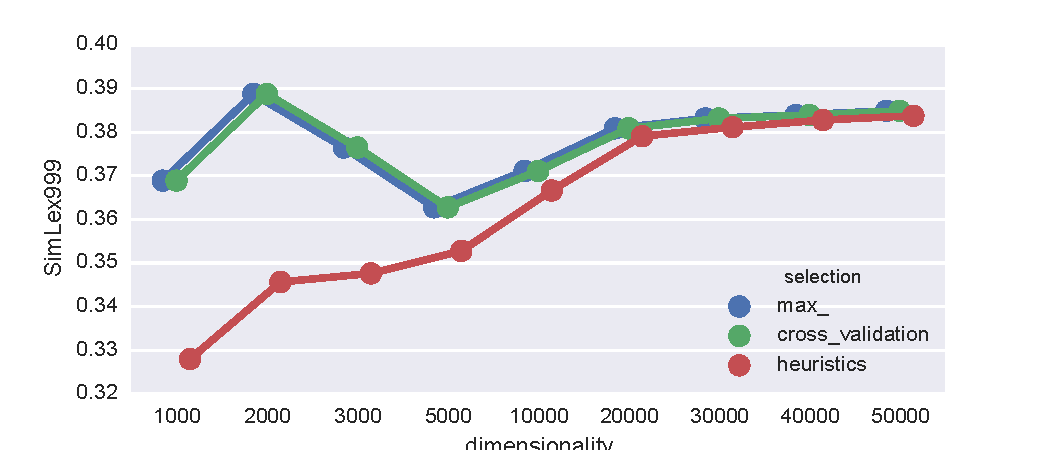
\includegraphics[width=0.5\textwidth]{supplement/figures/SimLex999-results}
  \caption{SimLex-999 results.}
  \label{fig:SimLex999-results}
\end{wrapfigure}

%%% Local Variables:
%%% mode: latex
%%% TeX-master: "../thesis"
%%% End:


Figure~\ref{fig:SimLex999-results} illustrates the results based on the best model selection and Table~\ref{tab:Simlex999-max-selection} shows the results together with picked parameters. Note that the maximum selection is identical with cross-validation: they pick the same models.

In general, model performance increases as the dimensionality increases. However, the best result of 0.389 is achieved with a 2000 dimensional space, this could, however, be an example of overfitting. Model performance becomes stable for dimensions greater than 20000.

For spaces with dimensionality less than 5000 \texttt{freq} 1 and inner product yield best results. Otherwise, cosine with \logNSCPMI/, smoothing $\alpha=0.75$ and shifting $k=0.7$ gives the best results. This supports our hypotheses H\ref{hyp:freq}, H\ref{hyp:cds} and H\ref{hyp:neg}.

\begin{table}
  \centering

  \begin{tabular}{rrlllrl}
\toprule
 dimensionality &  SimLex999 &  freq &  discr &     cds &  neg &     similarity \\
\midrule
           1\,000 &      0.369 &     1 &   spmi &       1 &  0.2 &  inner\_product \\
           2\,000 &      0.389 &     1 &  scpmi &  global &  0.7 &  inner\_product \\
           3\,000 &      0.376 &     1 &   spmi &    0.75 &  0.2 &  inner\_product \\
           5\,000 &      0.363 &  logn &  scpmi &  global &  1.0 &            cos \\
          10\,000 &      0.371 &  logn &  scpmi &       1 &  0.7 &            cos \\
          20\,000 &      0.381 &  logn &  scpmi &    0.75 &  0.7 &            cos \\
          30\,000 &      0.383 &  logn &  scpmi &    0.75 &  0.7 &            cos \\
          40\,000 &      0.384 &  logn &  scpmi &    0.75 &  0.7 &            cos \\
          50\,000 &      0.385 &  logn &  scpmi &    0.75 &  0.7 &            cos \\
\bottomrule
\end{tabular}


  \caption{SimLex-999 Max selection.}
  \label{tab:Simlex999-max-selection}
\end{table}


\subsection{Heuristics}
\label{sec:heuristics-simlex}

\begin{wraptable}[8]{O}{0.5\textwidth}
  \vspace{-1em}
  \centering

  \begin{tabular}{lr}
\toprule
      parameter &  partial $R^2$ \\
\midrule
     similarity &       0.38 \\
           freq &       0.27 \\
            neg &       0.24 \\
 dimensionality &       0.08 \\
          discr &       0.08 \\
            cds &       0.06 \\
\bottomrule
\end{tabular}


  \caption{SimLex-999 feature ablation}
  \label{tab:SimLex999-ablation}
\end{wraptable}


% \begin{figure}

  \centering

  \begin{subfigure}[t]{0.49\textwidth}
    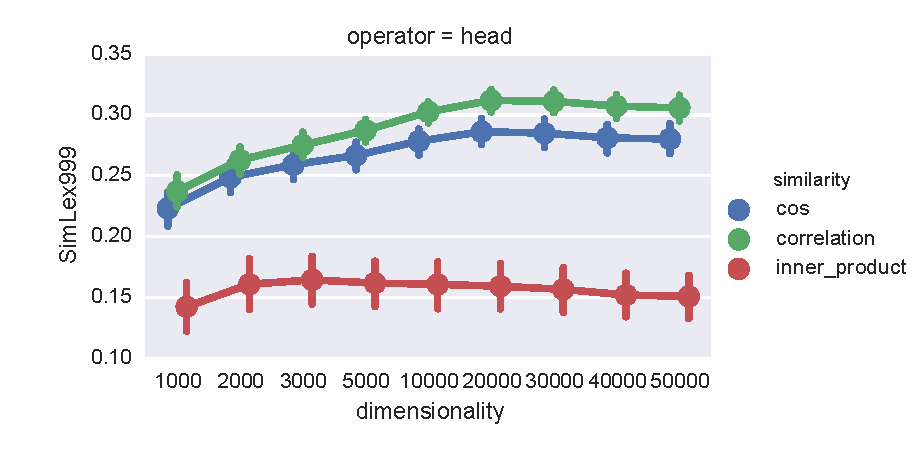
\includegraphics[width=\textwidth]{supplement/figures/SimLex999-interaction-similarity}
    \caption{similarity}
    \label{fig:SimLex999-interaction-similarity}
  \end{subfigure}
  \begin{subfigure}[t]{0.49\textwidth}
    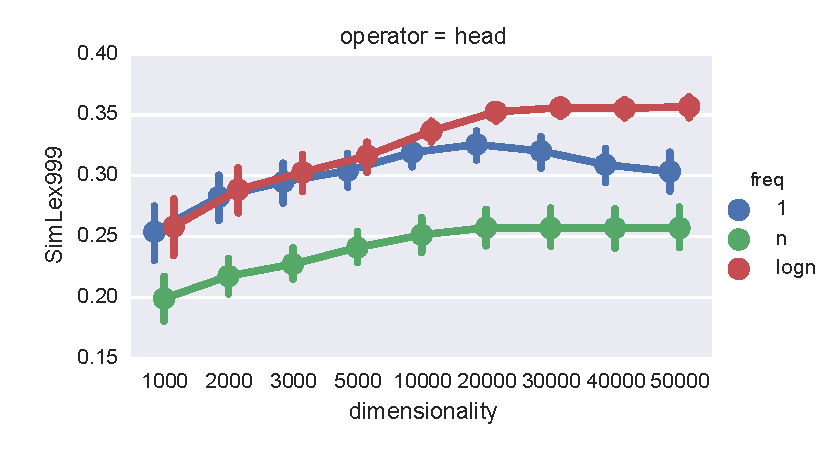
\includegraphics[width=\textwidth]{supplement/figures/SimLex999-interaction-freq}
    \caption{\texttt{freq}}
    \label{fig:SimLex999-interaction-freq}
  \end{subfigure}

  \begin{subfigure}[t]{0.49\textwidth}
    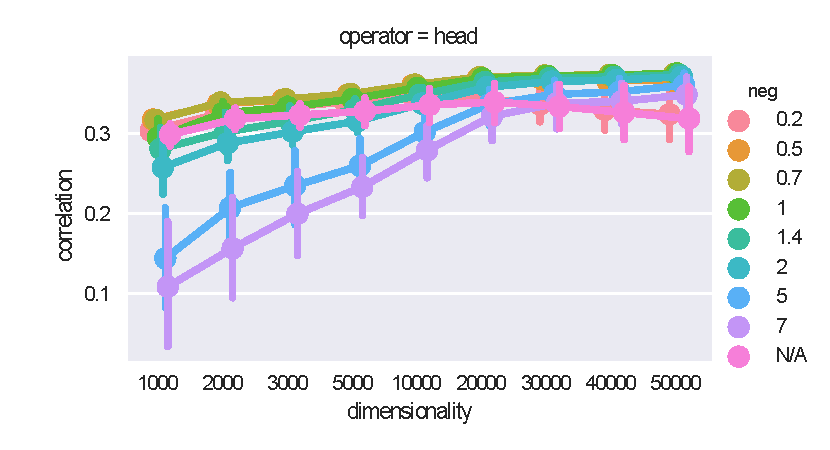
\includegraphics[width=\textwidth]{supplement/figures/SimLex999-interaction-neg}
    \caption{\texttt{neg}}
    \label{fig:SimLex999-interaction-neg}
  \end{subfigure}
  \begin{subfigure}[t]{0.49\textwidth}
    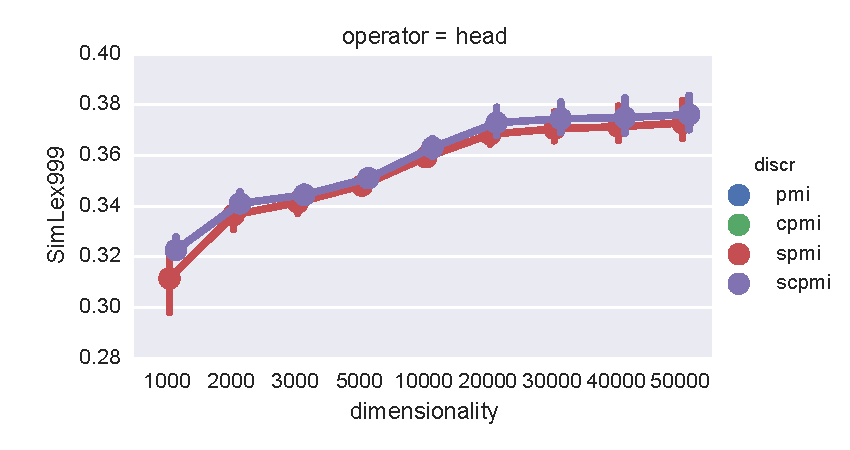
\includegraphics[width=\textwidth]{supplement/figures/SimLex999-interaction-discr}
    \caption{\texttt{discr}}
    \label{fig:SimLex999-interaction-discr}
  \end{subfigure}

  \begin{subfigure}[t]{0.49\textwidth}
    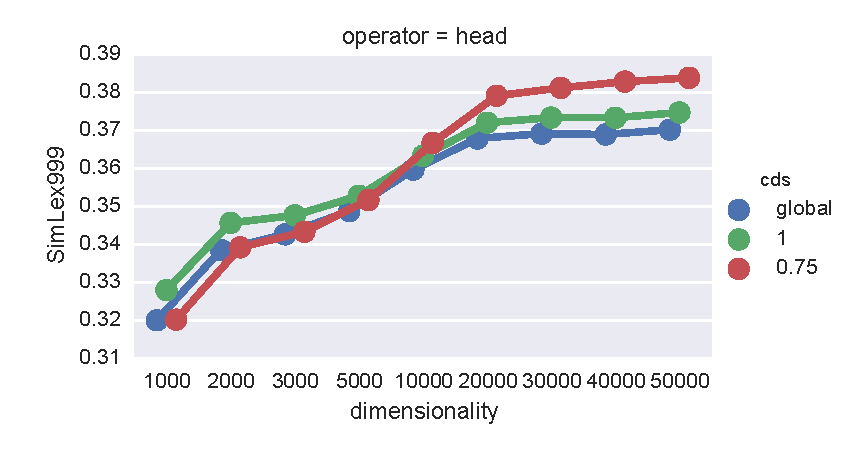
\includegraphics[width=\textwidth]{supplement/figures/SimLex999-interaction-cds}
    \caption{\texttt{cds}}
    \label{fig:SimLex999-interaction-cds}
  \end{subfigure}

  \caption{SimLex-999 parameter interaction. Parameters are shown in the order of their influence.}
  \label{fig:SimLex999-interaction}
\end{figure}

%%% Local Variables:
%%% mode: latex
%%% TeX-master: "../thesis"
%%% End:


The linear model achieves an adjusted $R^2$ of 0.867, indicating that the model is able to predict model performance based on parameter selection quite well. Table~\ref{tab:SimLex999-ablation} shows partial $R^2$ scores for parameters. The most influential parameters in decreasing order are similarity, \texttt{freq} and \texttt{neg}.

% \begin{wrapfigure}{O}{0.5\textwidth}
\begin{figure}
  % \vspace{-30pt}
  \centering

  \begin{subfigure}[t]{0.49\textwidth}
    \hspace{-20pt}
  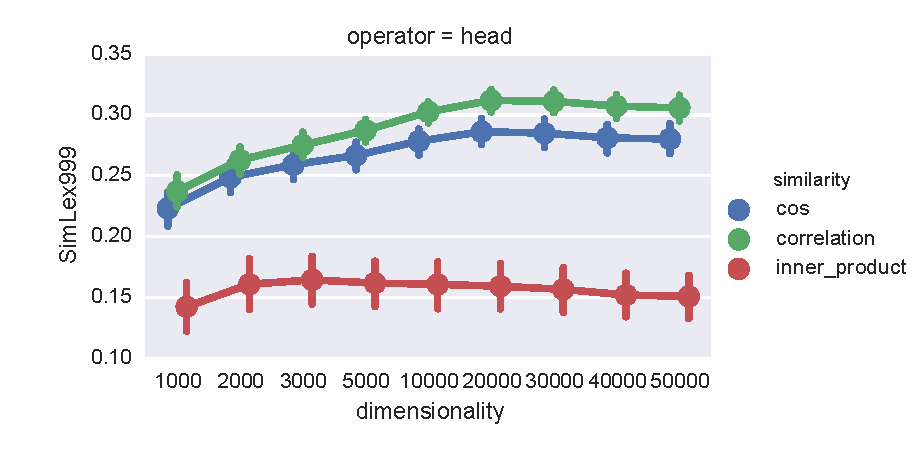
\includegraphics[width=1.1\textwidth]{supplement/figures/SimLex999-interaction-similarity}

  \caption{Similarity measure}
  \label{fig:SimLex999-similarity}

  \end{subfigure}
  \begin{subfigure}[t]{0.49\textwidth}

  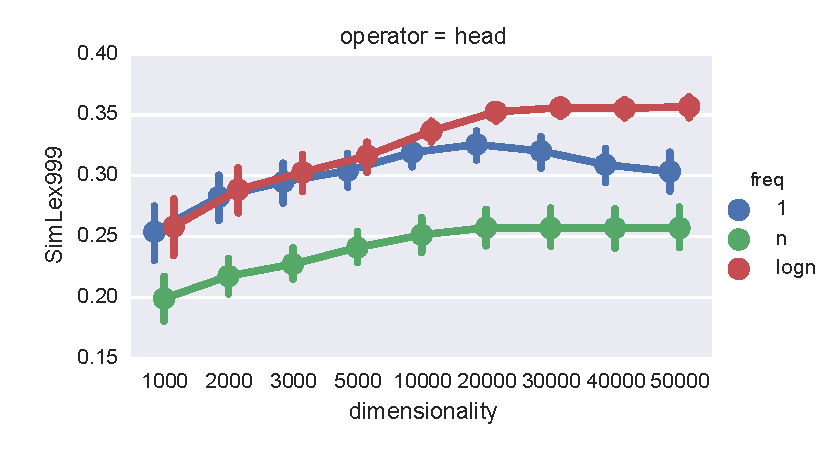
\includegraphics[width=\textwidth]{supplement/figures/SimLex999-interaction-freq}

  \caption{\texttt{freq}}
  \label{fig:SimLex999-freq}

  \end{subfigure}


  \begin{subfigure}[t]{0.49\textwidth}
  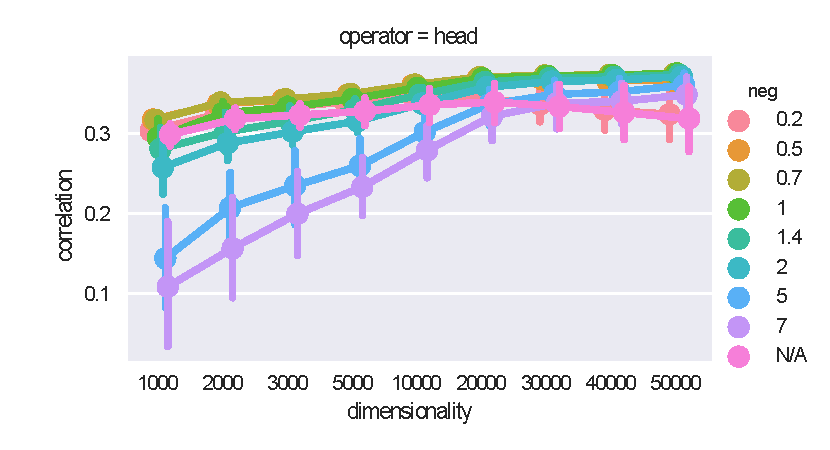
\includegraphics[width=\textwidth]{supplement/figures/SimLex999-interaction-neg}

  \caption{\texttt{neg}}
  \label{fig:SimLex999-neg}
  \end{subfigure}
  \begin{subfigure}[t]{0.49\textwidth}
  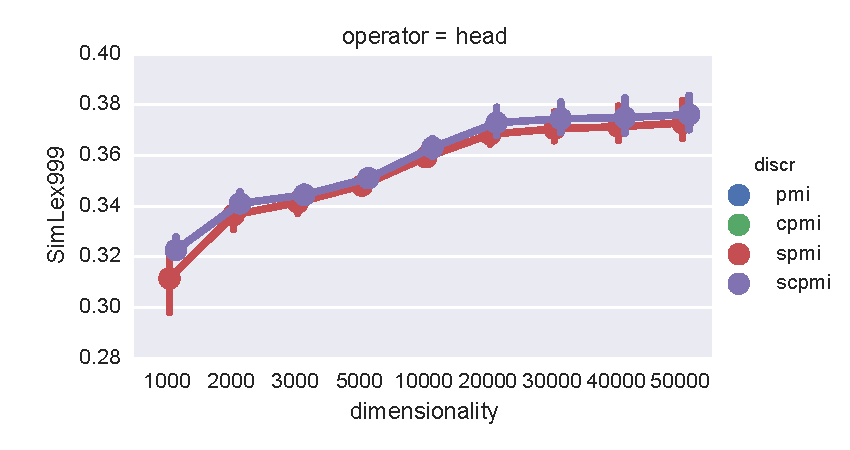
\includegraphics[width=\textwidth]{supplement/figures/SimLex999-interaction-discr}

  \caption{\texttt{discr}}
  \label{fig:SimLex999-discr}
  \end{subfigure}
  
  \caption[SimLex-999 influence of the similarity measure, \texttt{freq}, \texttt{neg} and \texttt{discr}]{SimLex-999 influence of the similarity measure, \texttt{freq}, \texttt{neg} and \texttt{discr}. Error bars indicate the 95\% confidence interval over the group of results.}
\end{figure}

Figure~\ref{fig:SimLex999-similarity} shows the average performance of similarity measures. Correlation outperforms all other measures for all dimensions and peaks at the dimensionality  of 20000 after correlation is chosen as the similarity measure. However, for $D \leq 5000$ the difference between correlation-based and cosine-based similarity measures is less than for $D > 5000$.

The influence of \texttt{freq}, the second parameter, is shown on Figure~\ref{fig:SimLex999-freq}. $\log n$ frequency outperforms other choices for all dimensions. After 20000 dimensions $\log n$'s performance stabilises: variance decreases and the performance stays constant. Taking into account that for $D \leq 5000$ there is little difference between $1$ and $\log n$, H\ref{hyp:freq} is supported in this case as well.

\begin{figure}[b]
% \begin{wrapfigure}{O}{0.5\textwidth}
  % \vspace{-30pt}
  \centering

  \begin{subfigure}[t]{0.49\textwidth}
  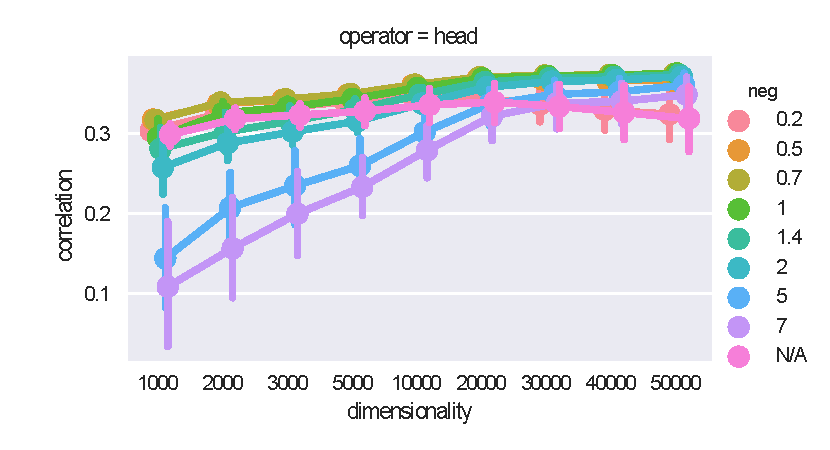
\includegraphics[width=\textwidth]{supplement/figures/SimLex999-interaction-neg}

  \caption{\texttt{neg}}
  \label{fig:SimLex999-neg}
  \end{subfigure}
  \begin{subfigure}[t]{0.49\textwidth}
  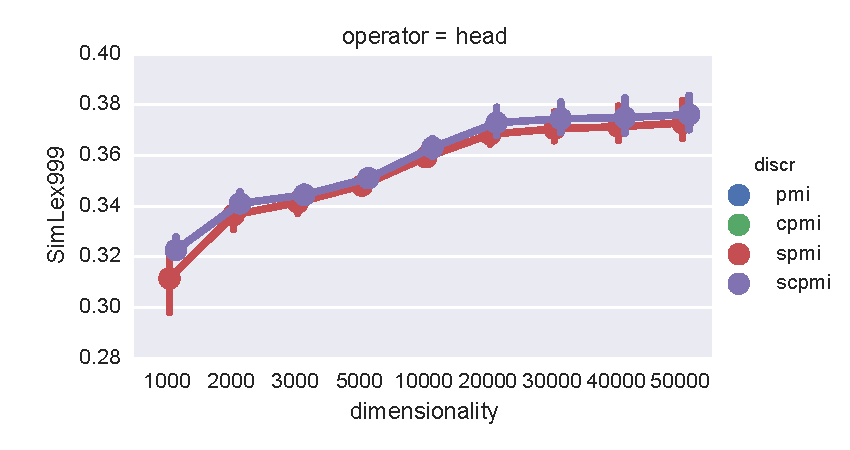
\includegraphics[width=\textwidth]{supplement/figures/SimLex999-interaction-discr}

  \caption{\texttt{discr}}
  \label{fig:SimLex999-discr}
  \end{subfigure}

  \caption{SimLex-999.}
\end{figure}

The third parameter \texttt{neg} of 0.7 shows the best performance (Figure~\ref{fig:SimLex999-neg}). However, there is little difference between models with dimensionality greater than 20000 (supporting H\ref{hyp:var} and H\ref{hyp:neg}), apart from the models that do not perform shifting, whose performance peaks at 20000 dimensions and decreases afterwards with increasing variance.

% \begin{figure}[h]
% \begin{wrapfigure}{O}{0.5\textwidth}
  % \vspace{-30pt}
  \centering

  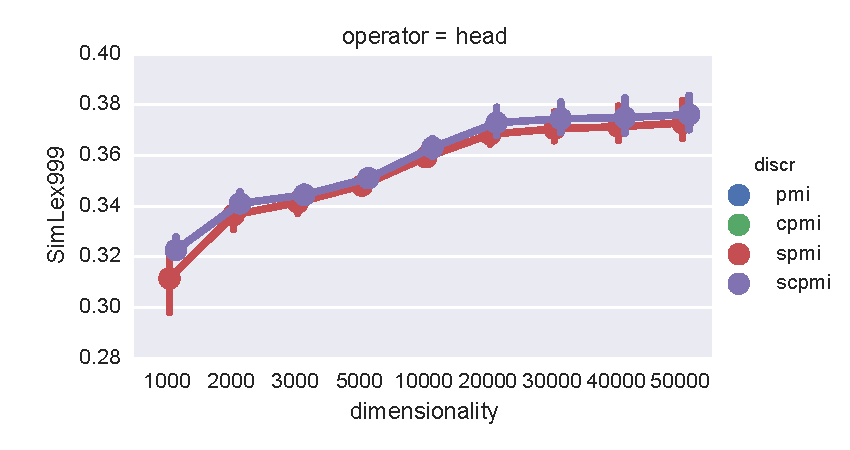
\includegraphics[width=0.5\textwidth]{supplement/figures/SimLex999-interaction-discr}

  \caption{SimLex-999 influence of \texttt{discr}. PMI and CPMI are not shown because at the step before models with shifting were chosen.}
  \label{fig:SimLex999-discr}
\end{figure}

There is little difference between SPMI and SCPMI performance with a little advantage to SCPMI (Figure~\ref{fig:SimLex999-discr}), supporting H\ref{hyp:lex-pmi-cpmi}.

% \begin{figure}[h]
\begin{wrapfigure}[5]{O}{0.5\textwidth}
  \vspace{-30pt}
  \centering

  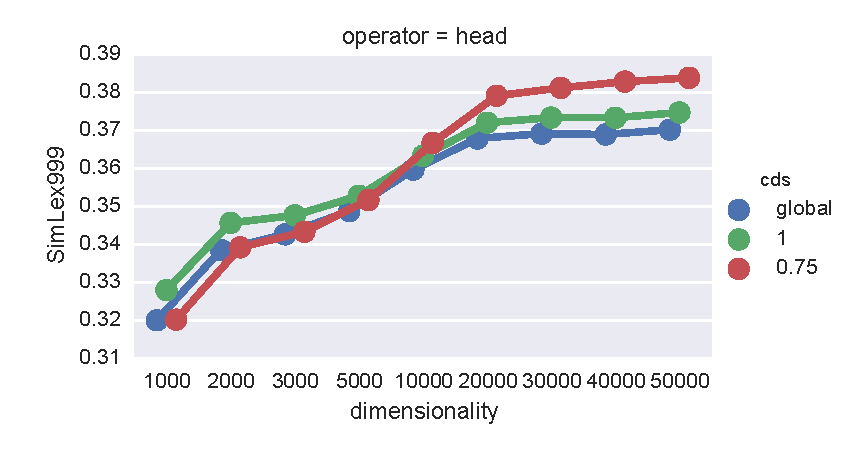
\includegraphics[width=0.5\textwidth]{supplement/figures/SimLex999-interaction-cds}
  \caption{SimLex-999 influence of \texttt{cds}.}
  \label{fig:SimLex999-cds}
\end{wrapfigure}

Finally, models benefit from context distribution smoothing, spaces with less than 10000 dimensions produce the best results with $\alpha = 1$, for spaces with higher dimensionality $\alpha = 0.75$ is the most advantageous (Figure~\ref{fig:SimLex999-cds}). This supports H\ref{hyp:cds} and replicates the results of \newcite{milajevs-sadrzadeh-purver:2016:ACL-SRW}.

\begin{table}
  \centering

  \begin{tabular}{rrlllll}
\toprule
 dimensionality &  SimLex999 &  freq &  discr &   cds &  neg &   similarity \\
\midrule
           1\,000 &      0.328 &  logn &  scpmi &     1 &  0.7 &  correlation \\
           2\,000 &      0.346 &  logn &  scpmi &     1 &  0.7 &  correlation \\
           3\,000 &      0.348 &  logn &  scpmi &     1 &  0.7 &  correlation \\
           5\,000 &      0.353 &  logn &  scpmi &     1 &  0.7 &  correlation \\
          10\,000 &      0.367 &  logn &  scpmi &  0.75 &  0.7 &  correlation \\
          20\,000 &      0.379 &  logn &  scpmi &  0.75 &  0.7 &  correlation \\
          30\,000 &      0.381 &  logn &  scpmi &  0.75 &  0.7 &  correlation \\
          40\,000 &      0.383 &  logn &  scpmi &  0.75 &  0.7 &  correlation \\
          \textbf{50\,000} &      \textbf{0.384} &  \textbf{logn} &  \textbf{scpmi} &  \textbf{0.75} &  \textbf{0.7} &  \textbf{correlation} \\
\bottomrule
\end{tabular}


  \caption{SimLex-999 selection based on heuristics. The highest value is 0.384.
  The values that are grater than 0.361 are indistinguishable from the highest score.}
  \label{tab:Simlex999-heuristics-selection}
\end{table}


\subsection{Difference between Max selection and heuristics on SimLex-999}

As expected, manual parameter selection is more homogeneous as Table~\ref{tab:Simlex999-heuristics-selection} shows. Both selection models agree on parameters for highly dimensional spaces ($D \geq 2000$), with an exception of similarity: Max selection prefers cosine, while manual prefers correlation based similarity measure. Because of this, manual selection does not pick the best result of the 2000 dimensional model, but at 50000 dimensions a model selected manually scores 0.001 lower: 0.384 versus 0.385 as also seen on Figure~\ref{fig:SimLex999-results}.

The average relative difference between Max selection and heuristics is 0.039, which is within the margin set by H\ref{hyp:10percent}.

\section{MEN}
\label{sec:men}

\subsection{Max selection}
\label{sec:max-selection-men}

\begin{figure}
  \centering

    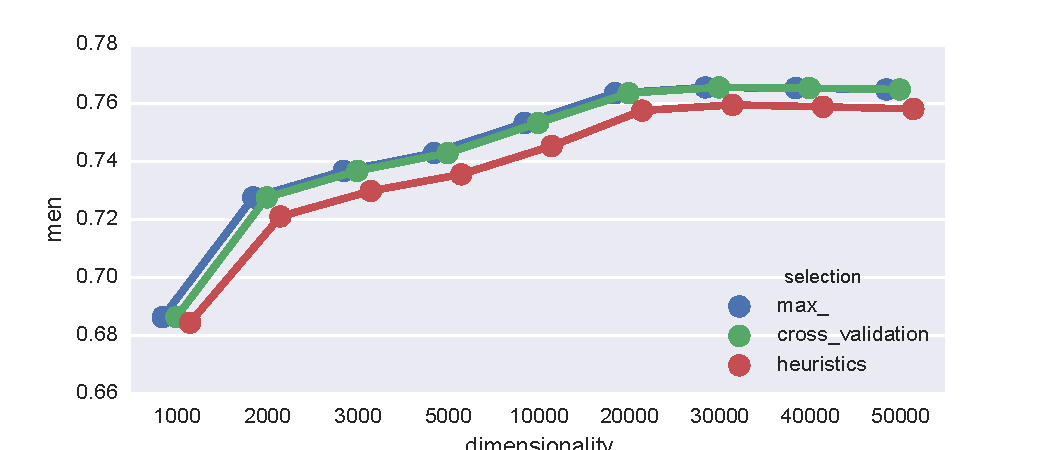
\includegraphics[width=0.5\textwidth]{supplement/figures/men-results}
  \caption{MEN results.}
  \label{fig:men-results}
\end{figure}

%%% Local Variables:
%%% mode: latex
%%% TeX-master: "../thesis"
%%% End:


Figure~\ref{fig:men-results} shows the selection results. Again, cross-validation results are identical with Max selection. Table~\ref{tab:men-max-selection} shows the results together with the selected models.

\begin{table}[b]
  \centering

  \begin{tabular}{rrlllrl}
\toprule
 dimensionality &    men &  freq &  discr &     cds &  neg &   similarity \\
\midrule
           1\,000 &  0.686 &     1 &  scpmi &  global &  1.4 &  correlation \\
           2\,000 &  0.728 &  logn &  scpmi &       1 &  0.7 &          cos \\
           3\,000 &  0.737 &  logn &  scpmi &       1 &  0.7 &          cos \\
           5\,000 &  0.743 &  logn &  scpmi &    0.75 &  0.7 &          cos \\
          10\,000 &  0.753 &  logn &  scpmi &    0.75 &  1.0 &  correlation \\
          20\,000 &  0.763 &  logn &  scpmi &    0.75 &  1.0 &  correlation \\
          \textbf{30\,000} &  \textbf{0.765} &  \textbf{logn} &  \textbf{scpmi} &    \textbf{0.75} &  \textbf{1.0} &  \textbf{correlation} \\
          \textbf{40\,000} &  \textbf{0.765} &  \textbf{logn} &  \textbf{scpmi} &    \textbf{0.75} &  \textbf{1.0} &  \textbf{correlation} \\
          \textbf{50\,000} &  \textbf{0.765} &  \textbf{logn} &  \textbf{scpmi} &    \textbf{0.75} &  \textbf{1.0} &  \textbf{correlation} \\
\bottomrule
\end{tabular}


  \caption{MEN Max selection}
  \label{tab:men-max-selection}
\end{table}


Model performance monotonically increases as the dimensionality increases. The highest score of 0.765 is achieved by 3 spaces with $D \geq 30000$, \logNSCPMI/, smoothed context distribution ($\alpha = 0.75$), shifted PMI values ($k = 1$) and the similarity measure based on correlation.

In comparison with SimLex-999, models with ``more extreme'' parameters give better results. For example, $\alpha = 0.75$ is the best for models tested on SimLex-999 with dimensionality starting with 20000, while for models tested on MEN, this parameter choice is the best starting with 5000. Similar behaviour is observed for \texttt{neg} and similarity. For highly dimensional spaces the switch from SimLex-999 to MEN changes the best \texttt{neg} choice from 0.7 to 1 and similarity from cosine to correlation. Such a switch of parameter choices might suggest the difference between \textit{relatedness} and \textit{similarity}, but it still supports H\ref{hyp:freq}, H\ref{hyp:cds} and H\ref{hyp:neg}.

\subsection{Heuristics}
\label{sec:heuristics-men}

\begin{wraptable}[11]{O}{0.5\textwidth}
  \vspace{1em}
  \centering

  \begin{tabular}{lr}
\toprule
      parameter &  partial $R^2$ \\
\midrule
            neg &  0.309 \\
           freq &  0.204 \\
     similarity &  0.183 \\
          discr &  0.119 \\
 dimensionality &  0.108 \\
            cds &  0.086 \\
\bottomrule
\end{tabular}


  \caption{MEN feature ablation}
  \label{tab:men-ablation}
\end{wraptable}

The linear model gives an adjusted $R^2$ of 0.733, which is lower than on SimLex-999, but is still high. Table~\ref{tab:men-ablation} shows partial $R^2$ scores for the explored parameters. The most influential parameter is \texttt{neg}, followed by \texttt{freq} and similarity. This is different in case of SimLex-999 where these parameters influence ``order'' is reversed.

\begin{figure}
% \begin{wrapfigure}{O}{0.5\textwidth}
  % \vspace{-30pt}
  \centering

  \begin{subfigure}[t]{0.49\textwidth}
    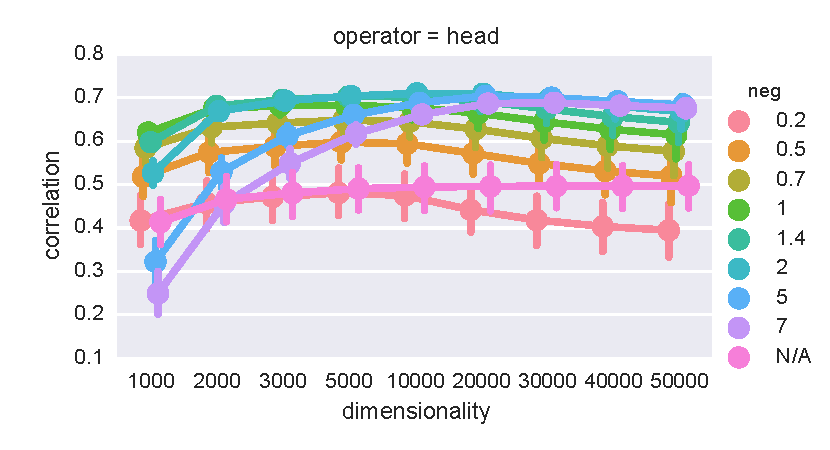
\includegraphics[width=\textwidth]{supplement/figures/men-interaction-neg}

  \caption{\texttt{neg}}
  \label{fig:men-neg}
  \end{subfigure}
  \begin{subfigure}[t]{0.49\textwidth}
    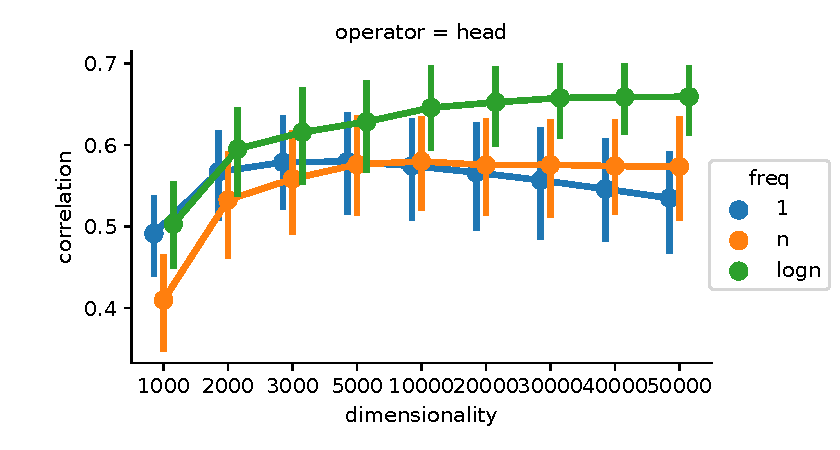
\includegraphics[width=\textwidth]{supplement/figures/men-interaction-freq}

  \caption{\texttt{freq}}
  \label{fig:men-freq}
  \end{subfigure}

  \caption{MEN.}
\end{figure}

\texttt{neg} with $k = 2$ is preferable for spaces with dimensionality less than 20000, for spaces with more dimensions,
$k = 5$ is more beneficial (Figure~\ref{fig:men-neg}). This replicates suggestions of \newcite{TACL570}). We, however, expect that for spaces with more than 500000 dimensions even higher values should be preferred. This contrasts with the heuristics derived from SimLex-999, where single \texttt{neg} value of 0.7 is chosen, but still complies with H\ref{hyp:neg}.

Regarding the frequency component, $\log n$ outperforms all other choices (Figure~\ref{fig:men-freq}). It is exactly the same behaviour as for heuristics based on SimLex-999 including the fact that $1$ and $\log n$ behave similarly for $D \leq 50000$, so H\ref{hyp:freq} is once again confirmed.

\begin{figure}[b]
% \begin{wrapfigure}{O}{0.5\textwidth}
  % \vspace{-30pt}
  \centering
  \begin{subfigure}[t]{0.49\textwidth}
    \hspace{-20pt}
    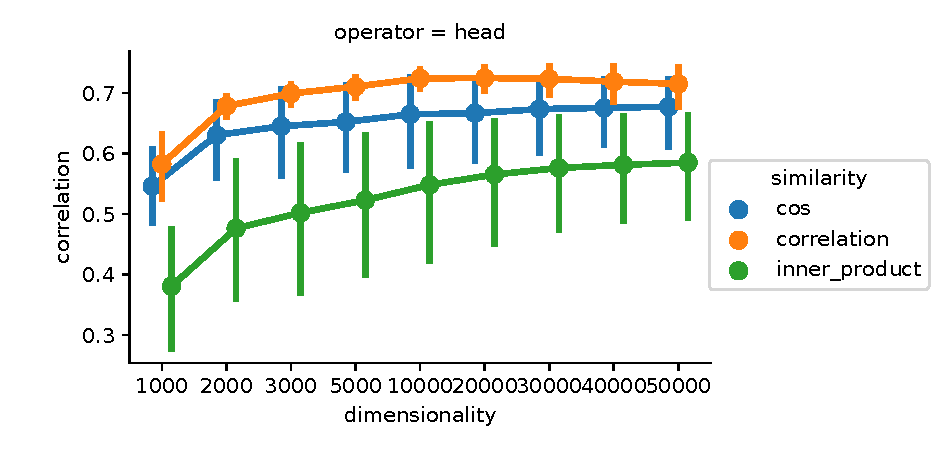
\includegraphics[width=1.1\textwidth]{supplement/figures/men-interaction-similarity}

  \caption{MEN influence of similarity.}
  \label{fig:men-similarity}
  \end{subfigure}
  \begin{subfigure}[t]{0.49\textwidth}
    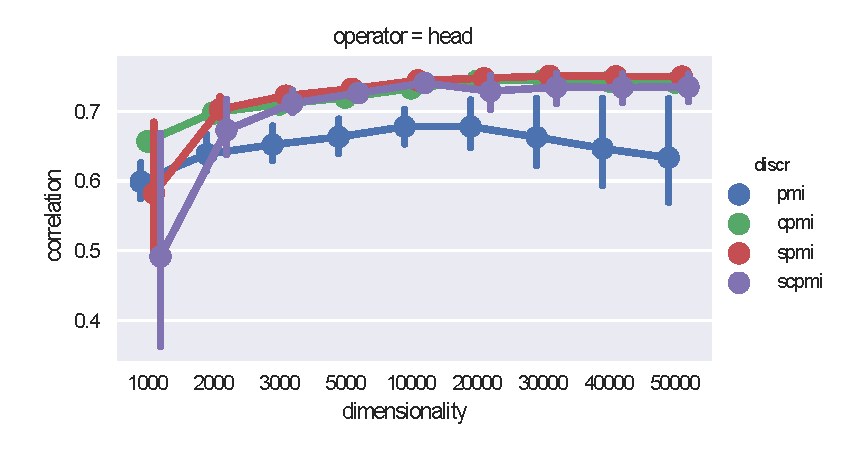
\includegraphics[width=\textwidth]{supplement/figures/men-interaction-discr}

  \caption{MEN influence of \texttt{discr}.}
  \label{fig:men-discr}
  \end{subfigure}
\end{figure}

Correlation is the preferred similarity measure (Figure~\ref{fig:men-similarity}), again this is inline with the choice based on SimLex-999.

SPMI is the preferred discriminativeness (Figure~\ref{fig:men-discr}), however it is closely followed by CPMI and SCPMI. This contrasts with SimLex-999, where SCPMI is preferred, however in both cases the difference between the two discriminativeness choices is minimal. This is inline with H\ref{hyp:lex-pmi-cpmi}.

\begin{figure}
%\begin{wrapfigure}[9]{O}{0.5\textwidth}
  % \vspace{-30pt}
  \centering

  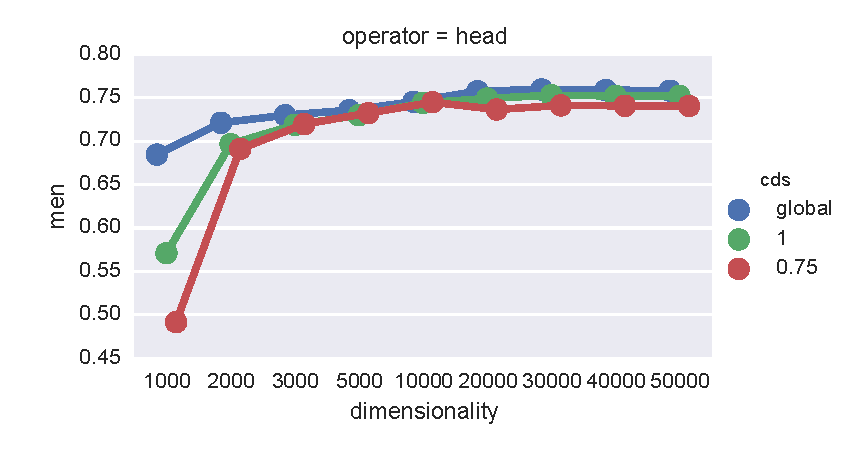
\includegraphics[width=0.5\textwidth]{supplement/figures/men-interaction-cds}

  \caption{MEN influence of \texttt{cds}}
  \label{fig:men-cds}
\end{figure}

Global context probability gives on average higher results for MEN (Figure~\ref{fig:men-cds}). Note, SimLex-999 prefers context distribution smoothing (Figure~\ref{fig:SimLex999-cds}). The difference in performance between local context probabilities and global context probabilities decreases as dimensionality increases, making a weak support of H\ref{hyp:cds}.

\subsection{Difference between Max selection and heuristics on MEN}

\begin{table}
  \centering

  \begin{tabular}{rrlllll}
\toprule
 dimensionality &    men &  freq & discr &     cds & neg &   similarity \\
\midrule
           1\,000 &  0.684 &  logn &  spmi &  global &   2 &  correlation \\
           2\,000 &  0.721 &  logn &  spmi &  global &   2 &  correlation \\
           3\,000 &  0.730 &  logn &  spmi &  global &   2 &  correlation \\
           5\,000 &  0.735 &  logn &  spmi &  global &   2 &  correlation \\
          10\,000 &  0.745 &  logn &  spmi &  global &   2 &  correlation \\
          20\,000 &  0.757 &  logn &  spmi &  global &   5 &  correlation \\
          \textbf{30\,000} &  \textbf{0.759} &  \textbf{logn} &  \textbf{spmi} &  \textbf{global} &   \textbf{5} &  \textbf{correlation} \\
          \textbf{40\,000} &  \textbf{0.759} &  \textbf{logn} &  \textbf{spmi} &  \textbf{global} &   \textbf{5} &  \textbf{correlation} \\
          50\,000 &  0.758 &  logn &  spmi &  global &   5 &  correlation \\
\bottomrule
\end{tabular}


  \caption{MEN selection based on heuristics. The highest value is 0.759. The
    values that are greater than 0.746 are indistinguishable from the highest score.}
  \label{tab:men-heuristics-selection}
\end{table}


The two selection procedures agree on fewer parameters than the ones bases on SimLex-999. Both agree on discrimination ($\log n$) and similarity score for spaces with dimensionality greater than 10000 (correlation). While SCPMI is chosen by Max selection, SPMI is preferred by the selection based on heuristics, however the difference between the two is minimal. In contrast to the Max selection, which chooses the models with context distribution smoothing, heuristics prefer models with global context probabilities. Also, heuristics pick models with higher shifting values $\alpha$ (2 and 5), in contrast to Max selection, where 0.7 and 1 are picked. Table~\ref{tab:men-heuristics-selection} summarises the parameter selection based on heuristics.

The average difference between Max selection and heuristics is 0.008, supporting H\ref{hyp:10percent}.

\section{Selected model transfer to another dataset}
\label{sec:select-model-transf}

\subsection{Difference between heuristics based on MEN and SimLex-999}

Heuristics based on MEN agree with ones bases on SimLex-999 on two parameters: frequency ($\log n$) and similarity (correlation). The methods disagree on \texttt{discr} (SCPMI versus SPMI, but the difference is neglectable as we expect by H\ref{hyp:lex-pmi-cpmi}), context distribution (smoothed versus global) and shifting parameter, for which higher values for MEN are preferred.

\subsection{From SimLex-999 to MEN}

\begin{figure}
  \centering

  \begin{subfigure}[t]{0.49\textwidth}
    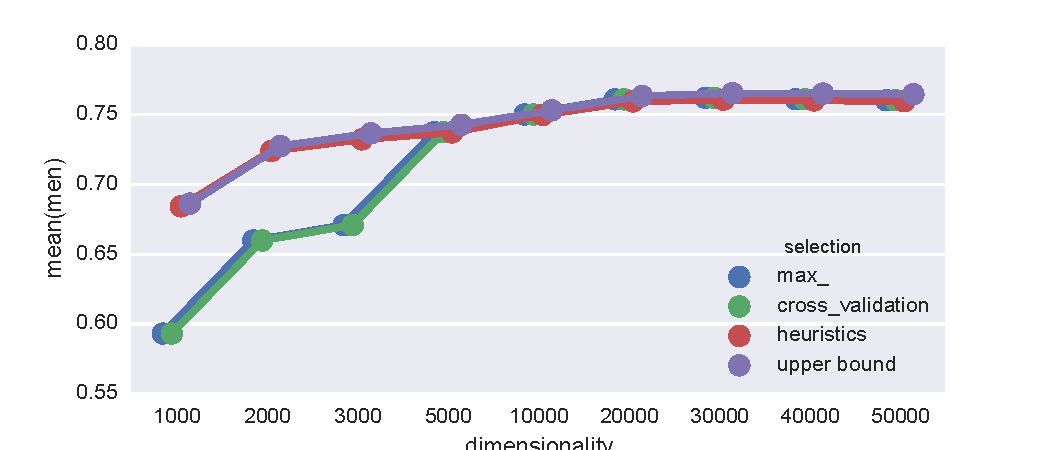
\includegraphics[width=\textwidth]{supplement/figures/SimLex999-transfer}
    \caption{Transfer from SimLex-999 to MEN}
    \label{fig:SimLex999-transfer}
  \end{subfigure}
  \begin{subfigure}[t]{0.49\textwidth}
    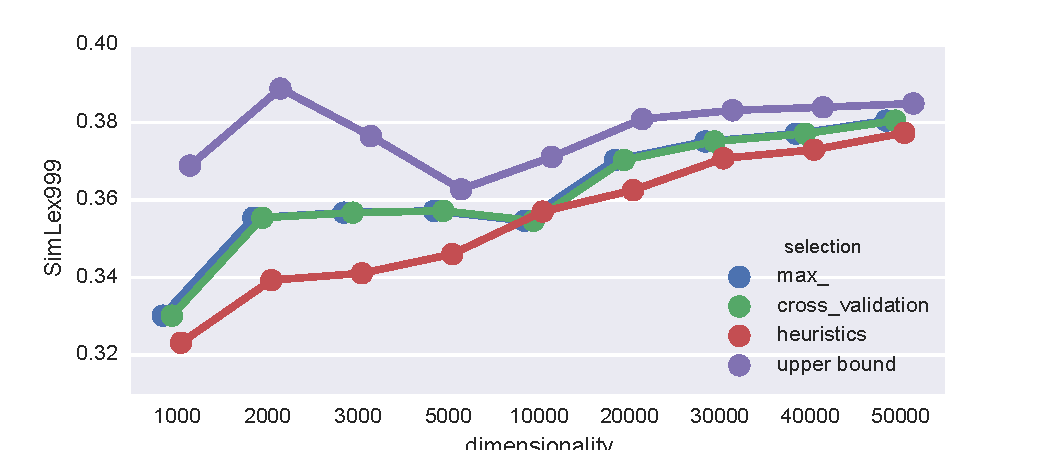
\includegraphics[width=\textwidth]{supplement/figures/men-transfer}
    \caption{Transfer from MEN to SimLex-999}
    \label{fig:men-transfer}
  \end{subfigure}

  \caption{Model transfer between lexical evaluation datasets}
  \label{fig:lexical-transfer}
\end{figure}

%%% Local Variables:
%%% mode: latex
%%% TeX-master: "../thesis"
%%% End:


The models selected using heuristics based on the SimLex-999 dataset perform well on MEN: for all dimensions the selected models are close to the best possible score (Figure~\ref{fig:SimLex999-transfer}). The average difference with the upper bound is 0.006, supporting H\ref{hyp:10percent}.

The max based selection comes close to the upper bound for models with dimensionality greater than 5000. The average difference with the upper bound is 0.039.

In this case, heuristic based selection leads to better performance than the Max based selection, supporting H\ref{hyp:overfitting}.

\subsection{From MEN to SimLex-999}

Heuristics transferred from MEN to SimLex-999 behave less efficient, they do not always outperform Max selection, though for highly dimensional spaces the difference decreases (Figure~\ref{fig:men-transfer}). The average difference is 0.062, which is ten times more than the transition from SimLex-999 to MEN, but still is within the limit set by H\ref{hyp:10percent}.

Max selection neither picks the best possible results when transferred from MEN to SimLex-999, however the average difference is lower: it is 0.042. This is similar to the transition in other direction.

Max based selection leads to better performance than the heuristics for MEN, making a case against H\ref{hyp:overfitting}.

\section{Universal parameter selection for lexical datasets}
\label{sec:universal-lexical-param-selection}

\begin{figure}[b]
  \centering

  \begin{subfigure}[t]{0.49\textwidth}
    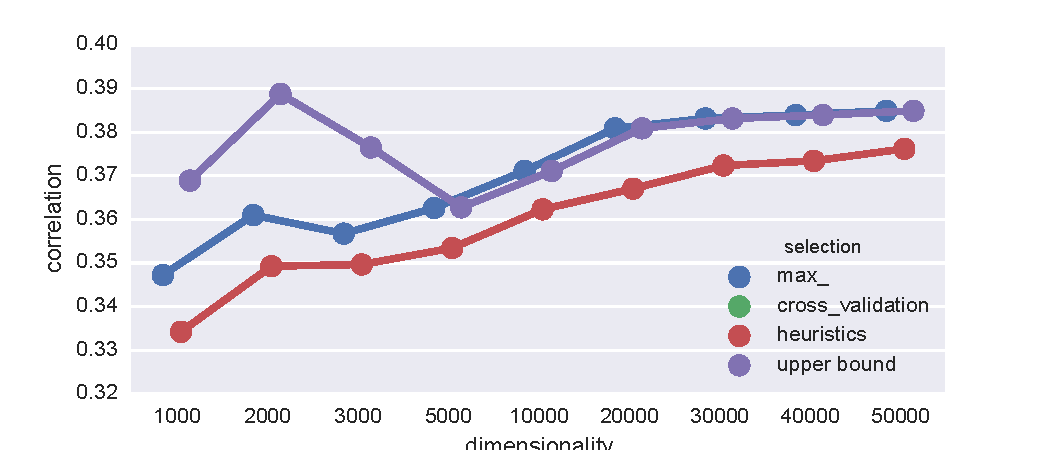
\includegraphics[width=\textwidth]{supplement/figures/lexical-results-SimLex999}
    \caption{SimLex-999}
    \label{fig:lexical-results-simlex}
  \end{subfigure}
  \begin{subfigure}[t]{0.49\textwidth}
    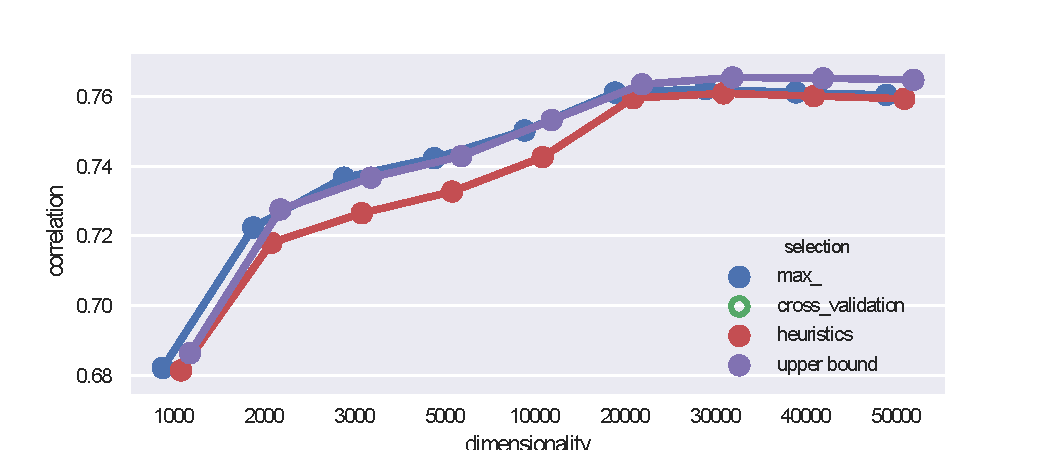
\includegraphics[width=\textwidth]{supplement/figures/lexical-results-men}
    \caption{MEN}
    \label{fig:lexical-results-men}
  \end{subfigure}

  \caption{Performance of models based on the selection over the average lexical performance}
  \label{fig:lexical-results}
\end{figure}

%%% Local Variables:
%%% mode: latex
%%% TeX-master: "../thesis"
%%% End:


Figure~\ref{fig:lexical-results} shows performance of the models based on the average of the normalised scores over SimLex-999 and MEN:
$$
\operatorname{score}_\mathit{lexical}(\mathit{model}) =%
\frac{1}{2}%
\frac{\operatorname{score}_\mathit{SimLex-999}(model)}%
{\max_m\operatorname{score}_\mathit{SimLex-999}(m)}%
+%
\frac{1}{2}%
\frac{\operatorname{score}_\mathit{MEN}(model)}%
{\max_m\operatorname{score}_\mathit{MEN}(m)}%
$$

The performance of the selected models on both datasets and the normalised average is shown on Table~\ref{tab:lexical-max-selection} (Max selection) and Table~\ref{tab:lexical-heuristics-selection} (selection based on heuristics).

\todo[inline]{Compare with Baroni and Levy.}

\subsection{Max selection}
\label{sec:max-selection}

In general, the more dimensions, the better the results are. The selection yields the best results at $D = 50000$ for SimLex-999 and at $D = 3000$ for MEN. While for SimLex-999,  the Max selection approaches the upper limit after 20000 dimensions; for MEN, it peaks and slightly deviates from the upper bound as the dimensionality increases.

The Max selection based on the combination of the two lexical datasets is closer to the Max selection based on SimLex-999 (Table~\ref{tab:Simlex999-max-selection}) than on MEN (Table~\ref{tab:men-max-selection}).

\begin{table}
  \centering

  \begin{tabular}{rrrrlllrl}
\toprule
 dimensionality &  SimLex999 &    men &  lexical &  freq &  discr &     cds &  neg & similarity \\
\midrule
           1\,000 &      0.347 &  0.682 &    0.892 &     1 &   spmi &  global &  1.4 &        cos \\
           2\,000 &      0.361 &  0.722 &    0.936 &  logn &  scpmi &  global &  1.0 &        cos \\
           3\,000 &      0.357 &  0.737 &    0.940 &  logn &  scpmi &       1 &  0.7 &        cos \\
           5\,000 &      \textbf{0.363} &  0.742 &    0.951 &  logn &  scpmi &       1 &  0.7 &        cos \\
          10\,000 &      \textbf{0.371} &  \textbf{0.750} &    0.967 &  logn &  scpmi &       1 &  0.7 &        cos \\
          20\,000 &      \textbf{0.381} &  \textbf{0.761} &    0.987 &  logn &  scpmi &    0.75 &  0.7 &        cos \\
          30\,000 &      \textbf{0.383} &  \textbe{0.762} &    0.991 &  logn &  scpmi &    0.75 &  0.7 &        cos \\
          40\,000 &      \textbf{0.384}  &  \textbf{0.761} &    0.991 &  logn &  scpmi &    0.75 &  0.7 &        cos \\
          50\,000 &     \textbe{ 0.385} &  \textbf{0.760} &    \textbe{0.992} &  logn &  scpmi &    0.75 &  0.7 &        cos \\
\bottomrule
\end{tabular}


  \caption[Lexical (combined SimLex-999 and MEN) Max selection]{Lexical (combined SimLex-999 and MEN) Max selection. For the
    individual dataset scores, the scores in bold are indistinguishable from the
  highest score. For SimLex-999, the highest score is 0.385 and the scores above
0.362 are indistinguishable. For MEN, the highest score is 0.762 and the scores
above 0.749 are indistinguishable. The highest combined score is 0.992 and the scores above 0.954 are indistinguishable.}
  \label{tab:lexical-max-selection}
\end{table}


\subsection{Heuristics}

\begin{wraptable}[13]{O}{0.5\textwidth}
  \vspace{3em}
  \centering

  \begin{tabular}{lr}
\toprule
      parameter &  partial $R^2$ \\
\midrule
     similarity &    0.299 \\
            neg &    0.280 \\
           freq &    0.231 \\
 dimensionality &    0.095 \\
          discr &    0.095 \\
            cds &    0.076 \\
\bottomrule
\end{tabular}


  \caption{Lexical feature ablation}
  \label{tab:lexical-ablation}
\end{wraptable}


The linear model achieves an adjusted $R^2$ of 0.817, which is less then $R^2 = 0.867$ of SimLex-999, but is greater than the $R^2 = 0.733$ of MEN. Table~\ref{tab:lexical-ablation} shows partial $R^2$ for each parameter, the most influential are similarity, \texttt{neg} and \texttt{freq}.

\begin{figure}[b]
% \begin{wrapfigure}{O}{0.5\textwidth}
  % \vspace{-30pt}
  \centering

  \begin{subfigure}[t]{0.49\textwidth}
    \hspace{-20pt}
    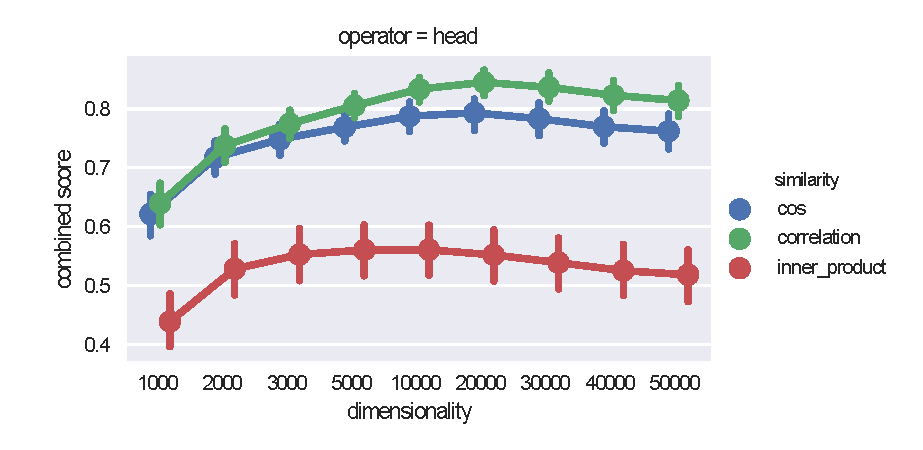
\includegraphics[width=1.1\textwidth]{supplement/figures/lexical-interaction-similarity}

    \caption{Similarity}
    \label{fig:lexical-similarity}
  \end{subfigure}
  \begin{subfigure}[t]{0.49\textwidth}
    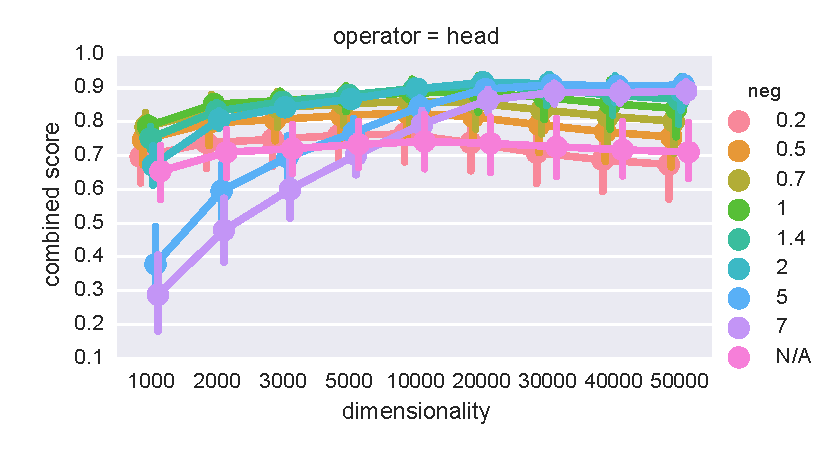
\includegraphics[width=\textwidth]{supplement/figures/lexical-interaction-neg}

    \caption{\texttt{neg}}
    \label{fig:lexical-neg}
  \end{subfigure}
  \caption{Lexical the influence of similarity and \texttt{neg}}
\end{figure}

Correlation is the similarity measure of choice (Figure~\ref{fig:lexical-similarity}). However, the difference between cosine and correlation is minimal for $D \leq 5000$.

For the models with dimensionality less than 20000 shifting should be used with $k = 1$, otherwise $k = 2$ is preferred (Figure~\ref{fig:lexical-neg}). This supports H\ref{hyp:neg}.

\begin{figure}[h]
% \begin{wrapfigure}{O}{0.5\textwidth}
  % \vspace{-30pt}
  \centering

  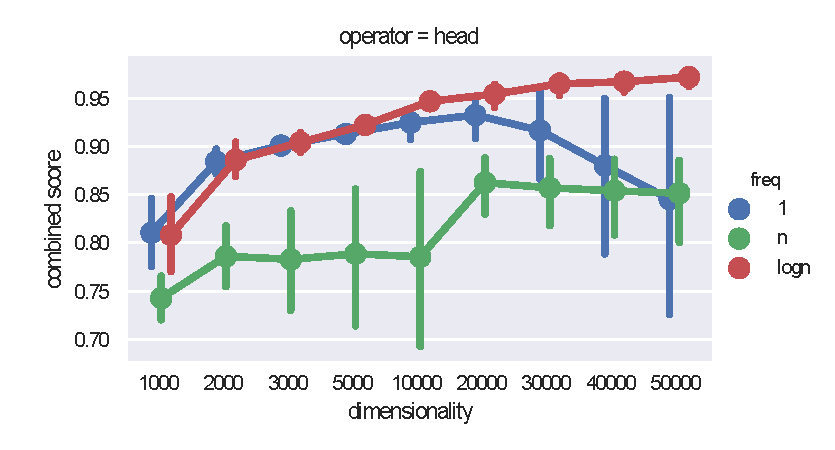
\includegraphics[width=0.5\textwidth]{supplement/figures/lexical-interaction-freq}

  \caption{Lexical influence of \texttt{freq}.}
  \label{fig:lexical-freq}
\end{figure}

$\log n$ on average performs the best as the frequency component (Figure~\ref{fig:lexical-freq}). But for $D \leq 5000$, 1 is also performs competitively to $\log n$, supporting H\ref{hyp:freq}.

SCPMI is the preferred discrimination component, but SPMI is very close to it (Figure~\ref{fig:lexical-discr}) backing up H\ref{hyp:lex-pmi-cpmi}.

% \begin{figure}[h]
\begin{wrapfigure}[7]{O}{0.5\textwidth}
  \vspace{-30pt}
  \centering

  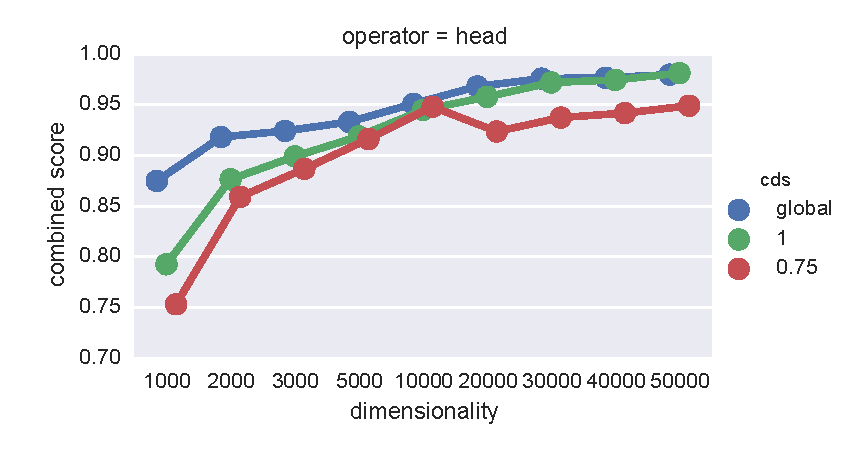
\includegraphics[width=0.5\textwidth]{supplement/figures/lexical-interaction-cds}

  \caption{Lexical influence of \texttt{cds}.}
  \label{fig:lexical-cds}
\end{wrapfigure}

Global context probabilities on average behave the best (Figure~\ref{fig:lexical-cds}). However, global context probabilities and local context probabilities with $\alpha = 1$ yield close results for $D > 10000$, giving support to H\ref{hyp:cds}.

\begin{table}
  \centering

  \begin{tabular}{rrrrlllll}
\toprule
 dimensionality &  SimLex999 &   men &  lexical &  freq &  discr &     cds & neg &   similarity \\
\midrule
           1\,000 &       0.33 &  0.68 &     0.87 &  logn &  scpmi &  global &   1 &  correlation \\
           2\,000 &       0.35 &  0.72 &     0.92 &  logn &  scpmi &  global &   1 &  correlation \\
           3\,000 &       0.35 &  0.73 &     0.92 &  logn &  scpmi &  global &   1 &  correlation \\
           5\,000 &       0.35 &  0.73 &     0.93 &  logn &  scpmi &  global &   1 &  correlation \\
          10\,000 &       0.36 &  0.74 &     0.95 &  logn &  scpmi &  global &   1 &  correlation \\
          20\,000 &       0.37 &  \textbf{0.76} &     0.97 &  logn &  scpmi &  global &   2 &  correlation \\
          30\,000 &       0.37 &  \textbf{0.76} &     \textbf{0.98} &  logn &  scpmi &  global &   2 &  correlation \\
          40\,000 &       0.37 &  \textbf{0.76} &     \textbf{0.98} &  logn &  scpmi &  global &   2 &  correlation \\
          50\,000 &       \textbf{0.38} &  \textbf{0.76} &     \textbf{0.98} &  logn &  scpmi &  global &   2 &  correlation \\
\bottomrule
\end{tabular}


  \caption{Lexical (combined SimLex-999 and MEN) selection based on heuristics.}
  \label{tab:lexical-heuristics-selection}
\end{table}


\subsection{Comparison with single dataset based selections}

Both selection methods mostly agree on frequency ($\log n$) and discriminativeness (SCPMI).

Context probability distribution smoothing varies between the selection methods, but follows the corresponding procedures based on MEN.

The Max based selection for \texttt{neg} follows the Max selection on SimLex-999.

Even though the similarity choice is different between the Max and heuristic selections, it is consistent with SimLex-999 in both cases and with MEN for the heuristic-based selection.

For the Max-based selection, the average difference is 0.020 on SimLex-999 and 0.004 for MEN.

For the heuristics-based selection, the average difference is 0.048 for SimLex-999 and 0.010 for MEN, which is within the 10\% limit set by H\ref{hyp:10percent}.

Max selection behaves better than the heuristics based on the average difference, but we can not check how well these two selections behave on other lexical datasets. This is an evidence against H\ref{hyp:overfitting}.

Based on the experiments, \logNSCPMI/ with shifting close to 1 is the quantification of choice for the lexical tasks, however more work needs to be done to find robust choice for context distribution smoothing and similarity measure.

\section{Conclusion}
\label{sec:conclusion-lexical}

Lexical experiments give support to the most of the stated hypotheses in Sections~\ref{sec:hypotheses} and \ref{sec:elab-hypoth-lexical}.

The optimal parameter choice depends on dimensionality (H\ref{hyp:dimen}). In particular, non constant frequency component (Section~\ref{sec:frequency-weighting}, H\ref{hyp:freq}), context distribution smoothing (Section~\ref{sec:cont-distr-smooth}, H\ref{hyp:cds}) and shifting (Section~\ref{sec:shifted-pmi}, H\ref{hyp:neg}) should be applied for spaces with $D \geq 10000$.

The switch at 10000 dimensions is a ``parameter sweet spot'' as parameter choice is not significant at these points, the most representable example is \texttt{cds} behaviour on SimLex-999 (Figure~\ref{fig:SimLex999-cds}. After that point performance either converges (supporting H\ref{hyp:var}), as in case of \texttt{neg} on SimLex-999 (Figure~\ref{fig:SimLex999-neg}), or there is one dominant choice, as for \texttt{freq} on SimLex-999 (Figure~\ref{fig:SimLex999-freq}).

As expected, we did not see a significant influence of the ``compression'' of the PMI values (H\ref{hyp:lex-pmi-cpmi}).

We could not find supporting evidence for H\ref{hyp:overfitting}, as Max-selected models performed well on transfer and both selection methods are within the 10\% difference margin to the highest result (H\ref{hyp:10percent}), suggesting that there indeed might be a universal vector space (H\ref{hyp:universal}).

We observed another regularity: cosine is a good similarity choice for low-dimensional spaces, but correlation is a better choice for highly-dimensional spaces.

\chapter{Similarity of sentences}
\label{sec:sentential}

\todo[inline]{Selection description: global best; best operator, its general behaviour, general behaviour of others; parameters.}

\section{Elaborated hypotheses}
\label{sec:elab-hypoth-comp}

As for the lexical experiments (Section~\ref{sec:elab-hypoth-lexical}), before reporting the results we refine some of our initial hypothesis (Section~\ref{sec:hypotheses}).

\begin{hyp}[H\ref{hyp:comp-pmi-cpmi}]
  \label{hyp:comp-pmi-cpmi}
  Compositional methods based on addition perform best with either PMI or SPMI, while methods that are based on multiplication should work best with CPMI and SCPMI.
\end{hyp}

The reason for that is the presence of negative values. In case of multiplication as a compositional operator, the sign of a vector component depends on the number of the corresponding negative components of the constituents. If the number of negative values is odd, then the resulting value will be negative. This makes the difference between 0.001 and -0.001 significant, while in the first case the value means that the co-occurrence pair is weakly associated, but in the second case the value means that the co-occurrence is weakly unassociated.

We also expect hypotheses related to PMI's Achilles heel (H\ref{hyp:freq}, H\ref{hyp:cds}, H\ref{hyp:neg}) to apply in the compositional case.

\begin{hyp}[H\ref{hyp:similarity}]
  \label{hyp:similarity}
  Cosine is an optimal similarity measure for low-dimensional spaces, while correlation is for highly-dimensional spaces.
\end{hyp}

We observed such behaviour in lexical tasks (Section~\ref{sec:conclusion-lexical}) and expect to see similar behaviour in compositional tasks.

\section{KS14}
\label{sec:ks14}

\subsection{Max selection}
\label{sec:max-selection-ks14}

\begin{figure}[b]
  \centering

    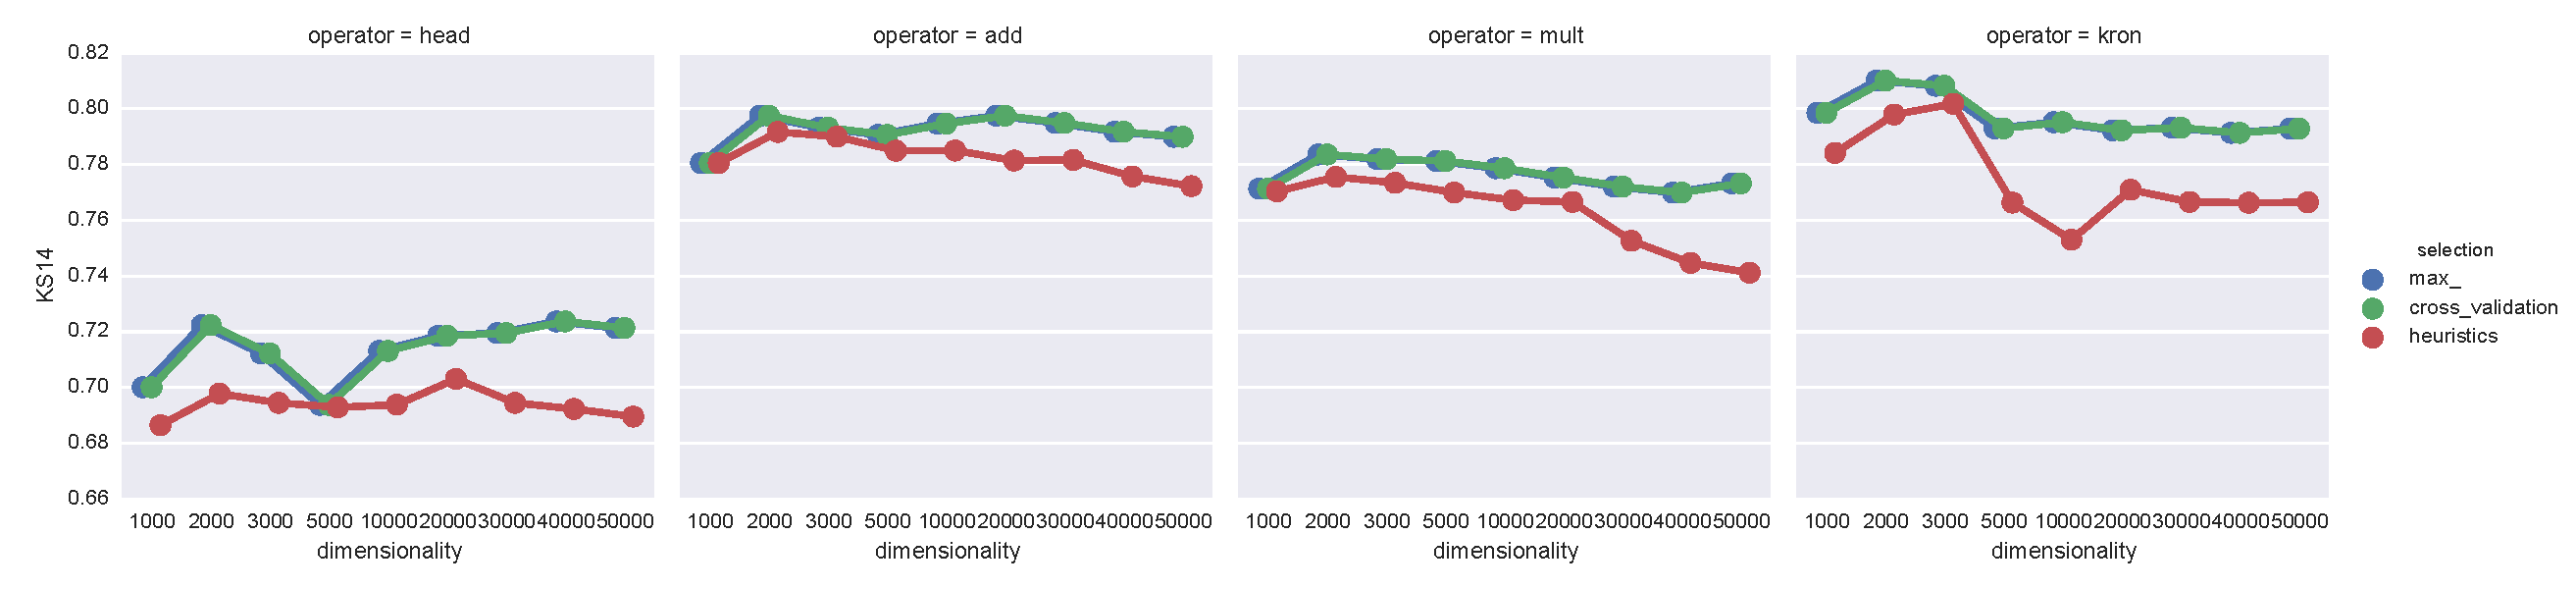
\includegraphics[width=\textwidth]{supplement/figures/ks14-results}
  \caption{KS14 results.}
  \label{fig:ks14-results}
\end{figure}

%%% Local Variables:
%%% mode: latex
%%% TeX-master: "../thesis"
%%% End:


Figure~\ref{fig:ks14-results} shows the performance of compositional model on the sentence similarity dataset KS14 \cite{kartsadrqpl2014}. All operators outperform the non-compositional \texttt{head} operator. Table~\ref{tab:ks14-max-selection} shows the performance of models selected by Max selection together with the selected parameters.

\todo[noline]{Significance test}
Kronecker with few thousand dimensions and correlation as the similarity measure gives the highest scores, supporting H\ref{hyp:order}. As the dimensionality increases, Kronecker performance stays constant. Addition is slightly better than multiplication, but the performance of both peaks at 2000 dimensions and decreases as the dimensionality increases.

\texttt{Head} parameters are similar to the lexical Max selection (Table~\ref{tab:lexical-max-selection}), with an exception of \texttt{neg}, where values similar to MEN (Table~\ref{tab:men-max-selection}) are chosen.

All compositional operators agree in the choice of \texttt{freq} ($\log n$), \texttt{discr} (SCPMI) and similarity (correlation, note that Kronecker was tested only with the inner product for $D > 3000$ because of limited computational resources).

Compositional operators perform best with constant \texttt{freq} of 1, in contrast to the lexical setting, where $\log n$ is more beneficial. This might be because during composition the $\log n$ term dominates over the PMI value and minimises its effect.

Local context probabilities perform better in compositional tasks. Multiplication benefits from the unsmoothed distribution probability, while highly dimensional models perform best with smoothing ($\alpha = 0.75$), supporting H\ref{hyp:cds}. The only exception are additive models with $D < 5000$, where global probabilities perform best.

For low dimensional spaces, addition performs best with sparse spaces ($k > 1$, $D < 5000$), but for high dimensional spaces, addition performs best  with dense spaces ($k = 0,7$, $D \geq 5000$), supporting H\ref{hyp:neg}.

Multiplication, independently of dimensionality, performs best with dense spaces ($k = 0.2$).

Kronecker, in contrast to addition, performs best with dense low dimensional models ($k = 0.2$, $D < 5000$) and sparser high dimensional models ($k = 0.7$, $D \geq 5000$). However, this difference might be explained by the change of the similarity measure, which is inner product for $D \geq 5000$.

\subsection{Heuristics}
\label{sec:heuristics}

\begin{wraptable}[11]{O}{0.5\textwidth}
  %\vspace{-10pt}
  \centering

  \begin{tabular}{lr}
\toprule
      parameter &  partial $R^2$ \\
\midrule
            neg &  0.331 \\
           freq &  0.307 \\
       operator &  0.305 \\
            cds &  0.136 \\
     similarity &  0.061 \\
          discr &  0.054 \\
 dimensionality &  0.034 \\
\bottomrule
\end{tabular}


  \caption{KS14 feature ablation}
  \label{tab:ks14-ablation}
\end{wraptable}


The linear model achieves an $R^2 = 0.794$. The partial $R^2$ are shown on Table~\ref{tab:ks14-ablation}. The most influential parameters are \texttt{neg}, \texttt{freq}, compositional operator and \texttt{cds}. Interestingly, similarity has much less influence on this compositional dataset than on lexical datasets, where for Sim-Lex-999 (Table~\ref{tab:SimLex999-ablation}) and combined (Table~\ref{tab:lexical-ablation}) it is the most influencing parameter. Also, note that dimensionality has the lowest partial $R^2$.

\subsubsection{Shifting}

\begin{figure}
% \begin{wrapfigure}{O}{0.5\textwidth}
  % \vspace{-30pt}
  \centering

  \begin{subfigure}[t]{\textwidth}
    \includegraphics[width=1.1\textwidth]{supplement/figures/ks14-interaction-neg}

  \caption{\texttt{neg}}
  \label{fig:ks14-neg}
  \end{subfigure}

  \begin{subfigure}[t]{\textwidth}
    \includegraphics[width=1.1\textwidth]{supplement/figures/ks14-interaction-freq}

  \caption{\texttt{freq}}
  \label{fig:ks14-freq}
  \end{subfigure}

  \caption{KS14.}
\end{figure}

For \texttt{head}, the best \texttt{neg} choice of $k$ is 1 for spaces with dimensionality less than 5000 (Figure~\ref{fig:ks14-neg}). For $5000 \leq D < 30000$, \texttt{head} behaves best with $k = 1.4$ and for $D \geq 3000$ \texttt{neg} should be set to 2.

For addition, spaces with $D < 20000$ should be used with $k = 1.4$, and with $k = 2$ otherwise.

For multiplication, there are three most beneficial choices: for $D < 10000$ $k = 0.5$, for $10000 \leq D < 30000$ $k = 0.7$ and, finally, for $D > 30000$ $k = 1$.

Kronecker shows similar behaviour of $k$ as dimensionality increases as multiplication, but prefers sparser spaces: for $D < 3000$ $k = 0.5$, for $3000 \leq D < 20000$ and $D \geq 20000$ $k = 1$.

All operators behave in accordance to H\ref{hyp:neg}.

\subsubsection{Frequency}
The best option of \texttt{freq} for \texttt{head} is $\log n$ (Figure~\ref{fig:ks14-freq}). The constant frequency 1 is very close $\log n$, but its performance declines for spaces with $D > 20000$.

For addition, frequency should be set to 1 for spaces with $D < 5000$ and to $\log n$ otherwise.

There is one choice of frequency for multiplication: 1, however $\log n$ behaves similarly to it for large values of $D$.

Kronecker follows addition with regard to \texttt{freq}, but the split point is $D = 10000$: low dimensional spaces should be used with constant frequency 1, and high dimensional spaces with $\log n$.

Therefore, H\ref{hyp:freq} is supported by this dataset.

\subsubsection{Context distribution smoothing}

\begin{figure}
% \begin{wrapfigure}{O}{0.5\textwidth}
  % \vspace{-30pt}
  \centering

  \begin{subfigure}[t]{\textwidth}
    \includegraphics[width=1.1\textwidth]{supplement/figures/ks14-interaction-cds}

  \caption{\texttt{cds}}
  \label{fig:ks14-cds}
  \end{subfigure}

  \begin{subfigure}[t]{\textwidth}
    \includegraphics[width=1.1\textwidth]{supplement/figures/ks14-interaction-similarity}

  \caption{\texttt{similarity}}
  \label{fig:ks14-similarity}
  \end{subfigure}

  \caption{KS14.}
\end{figure}

\texttt{Head} with spaces with dimensionality less than 20000 should be used with global probabilities, and more dimensional models should be used with smoothed local probabilities: $\alpha = 0.75$ (Figure~\ref{fig:ks14-cds}).

All other operators perform best with global context probability. Even though local context probability with $\alpha = 1$ is close to it, H\ref{hyp:cds} is not supported by this dataset.

\subsubsection{Similarity}
\texttt{Head} on spaces with $D < 20000$ performs best with cosine similarity, while more dimensional models prefer correlation as the similarity measure (Figure~\ref{fig:ks14-similarity}).

Other operators work best with correlation. Only addition supports H\ref{hyp:similarity}. In case of multiplication, correlation dominates over cosine even for small values of $D$. There is little to say about Kronecker, as it is tested only with the inner product for spaces with $D > 3000$ due to its computational complexity ($\mathcal{O}(n^2)$ with respect to the number of vector components).

\subsubsection{Discriminativeness}

\begin{figure}[b]
% \begin{wrapfigure}{O}{0.5\textwidth}
  % \vspace{-30pt}
  \centering

  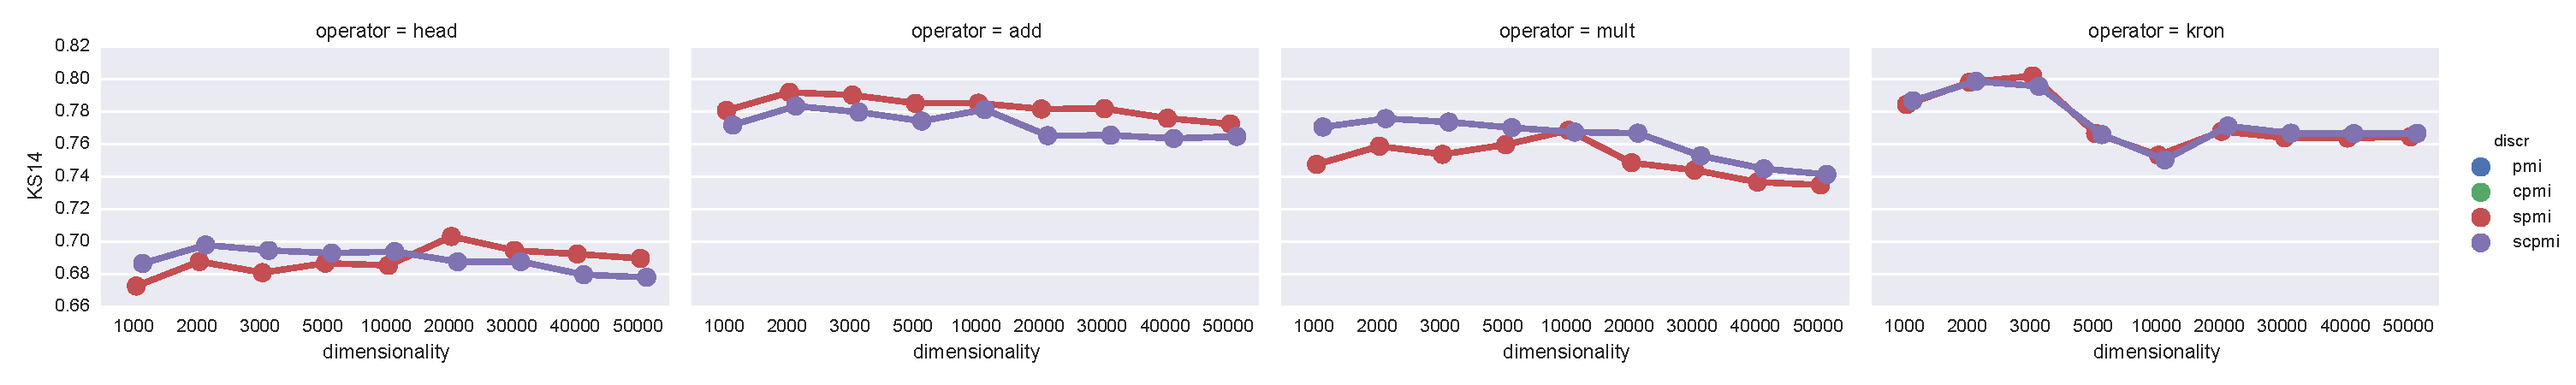
\includegraphics[width=1.1\textwidth]{supplement/figures/KS14-interaction-discr}

  \caption{KS14 influence of \texttt{discr}}
  \label{fig:ks14-discr}
\end{figure}

\texttt{Head} with $D < 20000$ prefers SCPMI as the discriminativeness weighting. SPMI is preferred otherwise (Figure~\ref{fig:ks14-discr}).

For addition, SPMI is the better choice. For multiplication, SCPMI is more beneficial, as expected by H\ref{hyp:comp-pmi-cpmi}.

For Kronecker, the two choices are very close to each other. However, for spaces with dimensionality less than 20000, SPMI is slightly better; for spaces with greater dimensionality, SCPMI is better.

\subsection{Difference between Max selection and heuristics on KS14}

Table~\ref{tab:ks14-heuristics-selection} shows the selection based on heuristics, which is more homogeneous than the selection based on the highest score (Table~\ref{tab:ks14-max-selection}). Both methods agree on the similarity choice (with an exception of \texttt{head}).

Multiplication agrees on the majority of parameters, but \texttt{cds} and \texttt{neg}. Local probabilities ($\alpha = 1$) and $k = 0.2$ give the highest score, while manual selection picked global context probabilities with \texttt{neg} in range on 0.5 to 1, in accordance to H\ref{hyp:neg}.

The average difference between Max and heuristic-based selections is 0.022. Per operator, the differences are: 0.028 \texttt{head}, 0.012 addition, 0.018 multiplication and 0.028 Kronecker. All the values are within the 10\% set by H\ref{hyp:10percent}.

\section{GS11}
\label{sec:gs11}

\todo[inline]{Mention \cite{hashimoto-tsuruoka:2016:P16-1}}

\subsection{Max selection}
\label{sec:max-selection-gs11}

\begin{figure}[b]
  \centering

    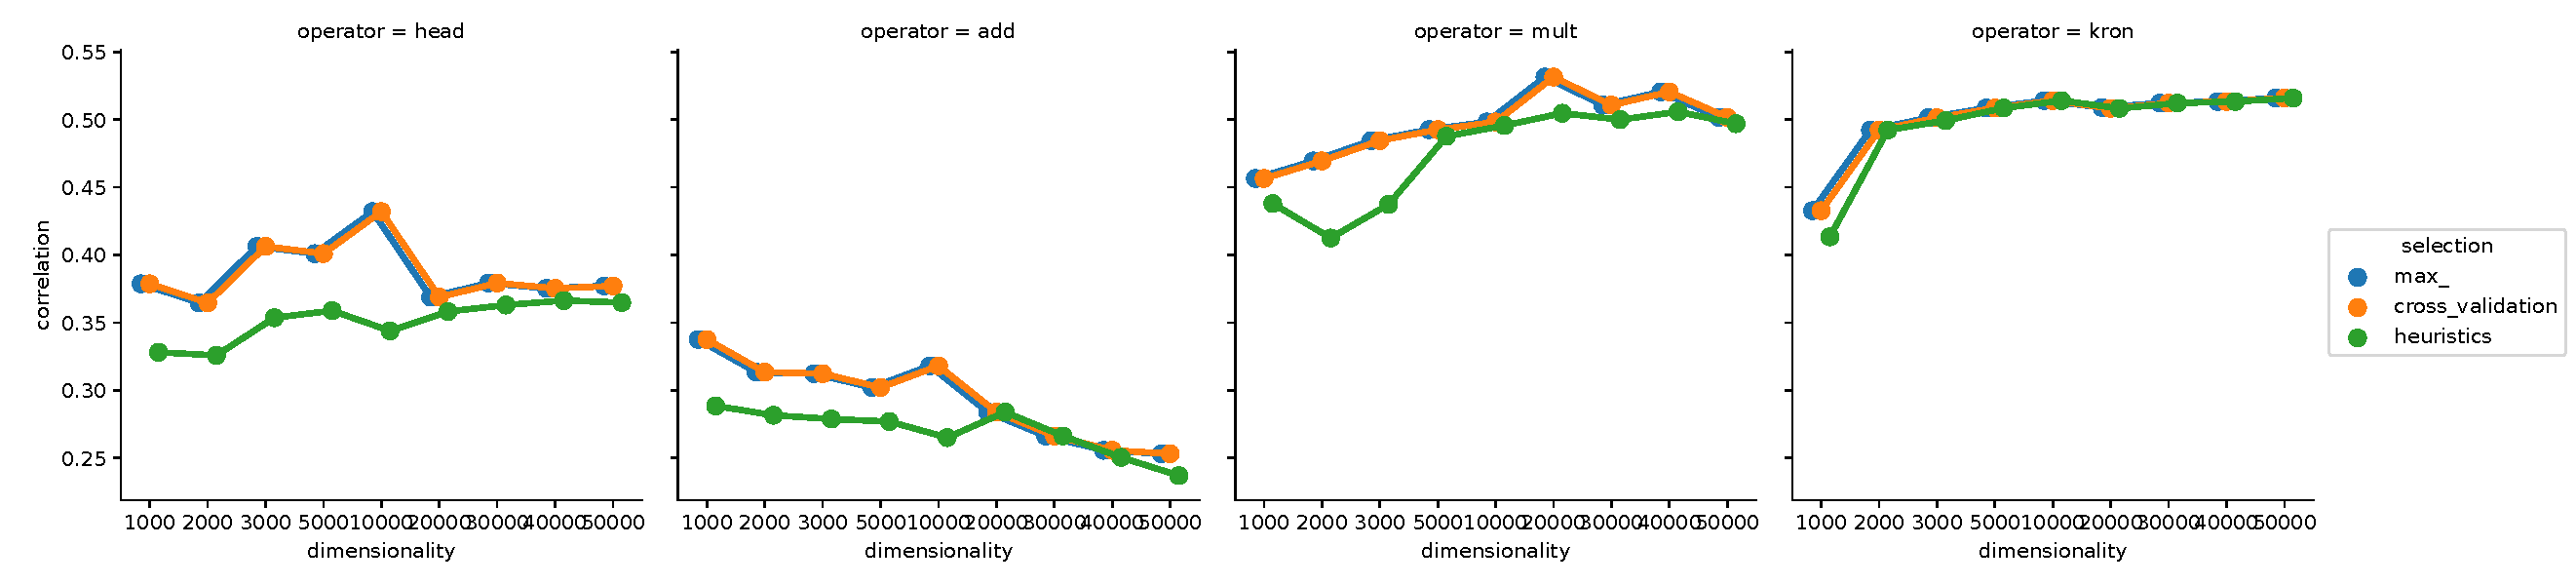
\includegraphics[width=\textwidth]{supplement/figures/gs11-results}
  \caption{GS11 results.}
  \label{fig:gs14-results}
\end{figure}

%%% Local Variables:
%%% mode: latex
%%% TeX-master: "../thesis"
%%% End:


Figure~\ref{fig:gs14-results} shows performance of the compositional models on the transitive verb disambiguation task \cite{Grefenstette:2011:ESC:2145432.2145580}. Table~\ref{tab:gs11-max-selection} shows the selected model performance together with chosen parameters.

Multiplication with 20000 dimensions gives the highest result of 0.532. Kronecker gets close with the score of 0.516 with $D = 50000$, giving no support to H\ref{hyp:order}. Addition does not outperform the \texttt{head} operator: addition scores 0.338, while \texttt{head}'s best performance is 0.432.

\texttt{Head}'s behaviour is unstable for dimensions less than 20000, and its best behaviour might be the case of overfitting similarly with SimLex-999. Models with dimensions greater than 20000 behave similarly to each other, even though the parameters are different.

In general, parameter selection is very different than the one based on KS14 (Table~\ref{tab:ks14-max-selection}). Compositional operators behave best with $\log n$ frequency, especially Kronecker. PMI often outperforms other discriminativeness components in case of \texttt{head} and addition. Global context probability estimation behaves better than local. Correlation is not always the best similarity measure.

Addition behaviour degrades as dimensionality increases, multiplication behaviour increases, but becomes unstable for spaces with high number of dimensions. Kronecker depends the least on the dimensionality. This gives no support to H\ref{hyp:var}.

Addition works best with dense models. Multiplication and Kronecker prefer dense low dimensional space and sparse high dimensional spaces, supporting H\ref{hyp:neg}.

\subsection{Heuristics}
\label{sec:heuristics-gs11}

\begin{wraptable}[8]{O}{0.5\textwidth}
% \begin{table}[b]
  \vspace{-4em}
  \centering
  \begin{tabular}{lr}
\toprule
      parameter &  partial $R^2$ \\
\midrule
       operator &  0.37 \\
           freq &  0.21 \\
            neg &  0.18 \\
     similarity &  0.09 \\
            cds &  0.05 \\
          discr &  0.04 \\
 dimensionality &  0.04 \\
\bottomrule
\end{tabular}


  \caption{GS11 feature ablation}
  \label{tab:gs11-ablation}
\end{wraptable}


The linear model achieves an $R^2 = 0.753$. The partial $R^2$ scores are shown on Table~\ref{tab:gs11-ablation}. The most influential parameters are a compositional operator, \texttt{freq} and \texttt{neg}. This is the same as in case of KS14, but in the reversed order (Table~\ref{tab:ks14-ablation}).


\subsubsection{Frequency}

\begin{figure}
% \begin{wrapfigure}{O}{0.5\textwidth}
  % \vspace{-30pt}
  \centering

  \begin{subfigure}[t]{\textwidth}
    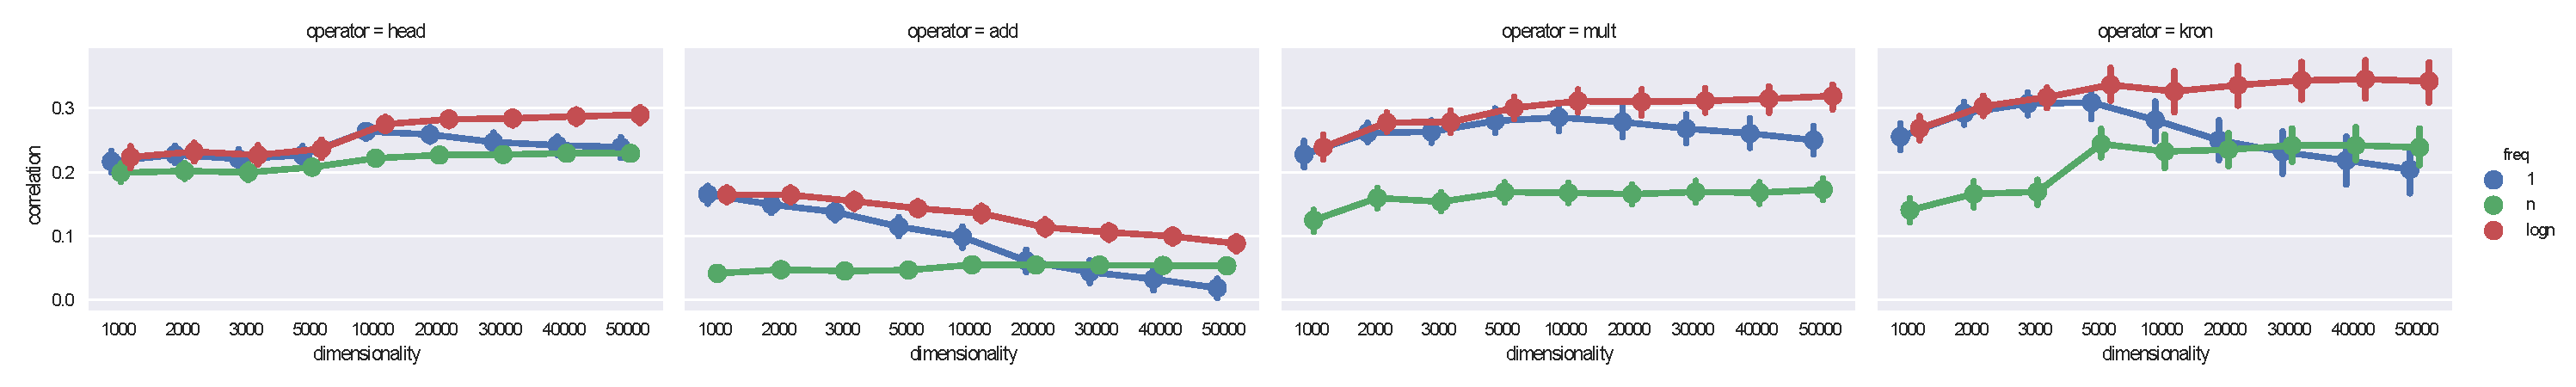
\includegraphics[width=1.1\textwidth]{supplement/figures/GS11-interaction-freq}

  \caption{\texttt{freq}}
  \label{fig:gs11-freq}
  \end{subfigure}

  \begin{subfigure}[t]{\textwidth}
    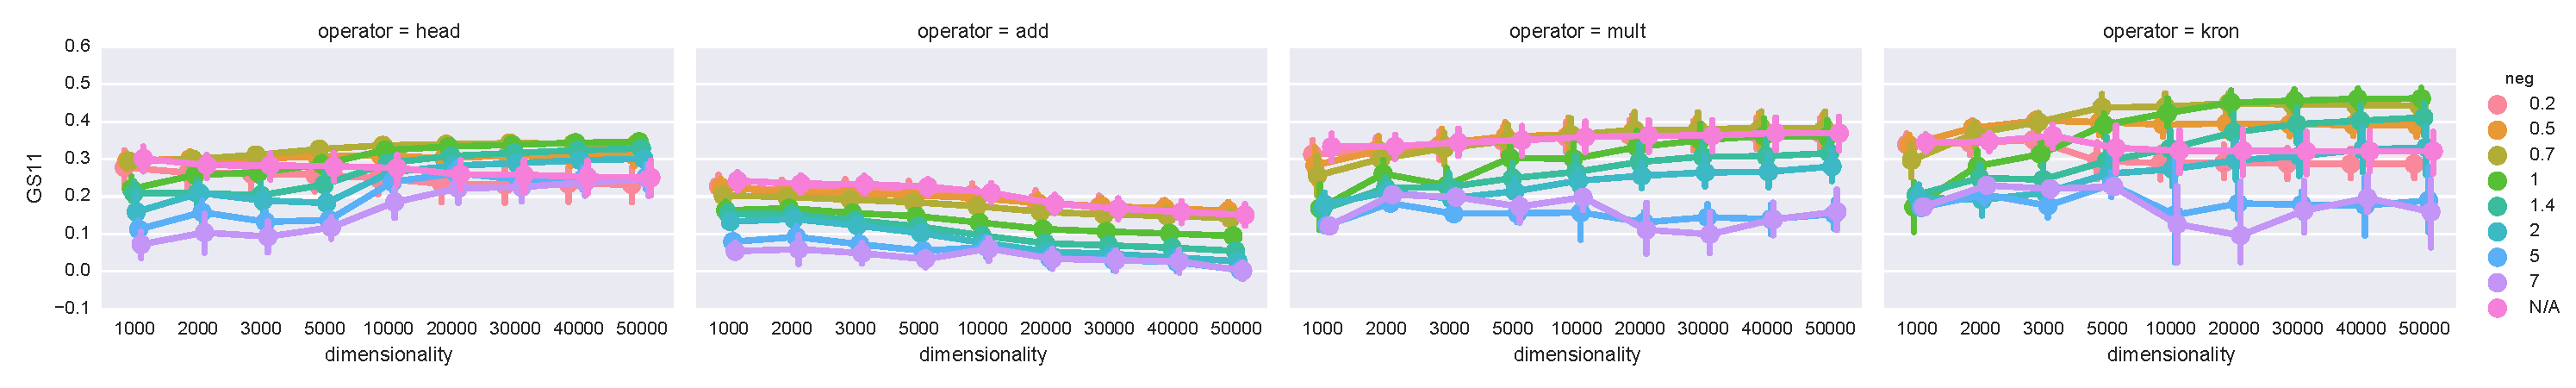
\includegraphics[width=1.1\textwidth]{supplement/figures/GS11-interaction-neg}

  \caption{\texttt{neg}}
  \label{fig:gs11-neg}
  \end{subfigure}

  \caption{GS11 influence of \texttt{freq} and \texttt{neg}}
\end{figure}


$\log n$ on average behaves best for all operators (Figure~\ref{fig:gs11-freq}). For $D \leq 5000$, 1 is also a good frequency choice, supporting H\ref{hyp:freq}.

\subsubsection{Shifting}

\texttt{Head} on average works best with shifted models. For models with dimensionality less than 3000, $k = 0.5$, otherwise $k = 0.7$ is more beneficial (Figure~\ref{fig:gs11-neg}).

For addition, models without shifting behaves best for $D < 20000$, however for more dimensional spaces, $k = 0.2$ should be preferred. This is a weak support of H\ref{hyp:neg}, because unshifted spaces can be seen as shifted with a very small $\alpha$ value.

Multiplication also works best with unshifted low dimensional spaces ($D < 5000$) and with $k = 0.7$ for high dimensional spaces, supporting H\ref{hyp:neg}.

Kronecker prefers shifting. For spaces with dimensionality less then 20000 $k = 0.7$ and $k = 1$ otherwise. This is according to H\ref{hyp:neg}.

\subsubsection{Similarity}

\begin{figure}
% \begin{wrapfigure}{O}{0.5\textwidth}
  % \vspace{-30pt}
  \centering

  \begin{subfigure}[t]{\textwidth}
    \includegraphics[width=1.1\textwidth]{supplement/figures/gs11-interaction-similarity}

  \caption{Similarity}
  \label{fig:gs11-similarity}
  \end{subfigure}

  \begin{subfigure}[t]{\textwidth}
    \includegraphics[width=1.1\textwidth]{supplement/figures/gs11-interaction-cds}

  \caption{\texttt{cds}}
  \label{fig:gs11-cds}
  \end{subfigure}

  \caption{GS11.}
\end{figure}


\texttt{Head} and multiplication work best with cosine similarity. Addition with correlation and Kronecker with inner product (Figure~\ref{fig:gs11-similarity}).

Addition strictly supports H\ref{hyp:similarity}, while multiplication supports it by behaving similarity with cosine and correlation.

\subsubsection{Context distribution smoothing}

\texttt{Head} with $D < 10000$ works best with global context probabilities. For more dimensional spaces, local context probabilities $\alpha = 1$ should be preferred (Figure~\ref{fig:gs11-cds}).

Addition works best with local probabilities. In the low dimensional case, when $D < 20000$, unsmoothed estimation ($\alpha = 1$) is preferred and $\alpha = 0.75$ should be chosen otherwise.

Multiplication works best with global context probabilities. Kronecker with smoothed local ($\alpha = 0.75$).

There is no support of H\ref{hyp:cds} because global context probabilities outperform other choices for multiplication, addition behaves the same with all options and Kronecker works best with $\alpha = 0.75$.

\subsubsection{Discriminativeness}

\begin{figure}[b]
% \begin{wrapfigure}{O}{0.5\textwidth}
  % \vspace{-30pt}
  \centering

  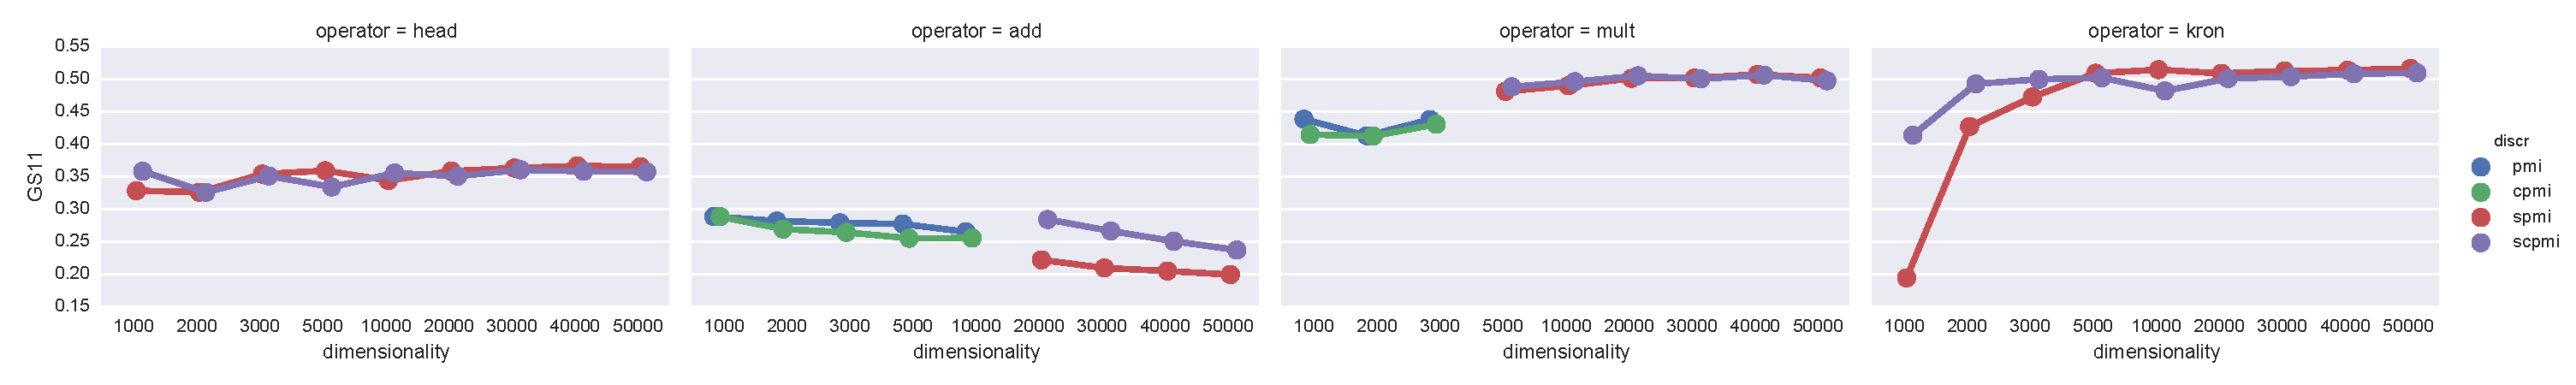
\includegraphics[width=1.1\textwidth]{supplement/figures/GS11-interaction-discr}

  \caption{GS11 \texttt{discr}}
  \label{fig:gs11-discr}
\end{figure}


\texttt{Head} works best with SPMI, but SCPMI is very close (Figure~\ref{fig:gs11-discr}).

Addition works best with PMI for $D < 20000$ and SCPMI otherwise.

Multiplication is similar to addition that it prefers PMI in the low dimensional case and SCPMI in the high dimensional case, but the change happens at 5000 dimensions.

Kronecker with less than 5000 dimensions prefers SCPMI and SPMI otherwise.

This dataset does not give evidence to support H\ref{hyp:comp-pmi-cpmi}.

\subsection{Difference between Max selection and heuristics on GS11}

Only logarithmic frequency component ($\log n$) was chosen by heuristics (Table~\ref{tab:gs11-heuristics-selection}), while there is a mix of 1 and $\log n$ in the Max selection (Table~\ref{tab:gs11-max-selection}).

Kronecker and most of multiplication discriminativeness choices agree, while for \texttt{head} and addition there is little agreement between parameter selection. Same goes for context distribution smoothing and shifting.

Similarity choice is the same for Kronecker and addition, but \texttt{head} and multiplication---according to heuristics---should be used with cosine similarity, while there is no single metric that leads to maximum performance.

The overall average normalised difference in results between Max and heuristic-based selections is 0.054. Per operator, the differences are: 0.090 \texttt{head}, 0.077 addition, 0.043 multiplication and 0.006 Kronecker. All the values are within the 10\% boundary (H\ref{hyp:10percent}).

\section{PhraseRel}
\label{sec:phraserel-experiment}

\subsection{Max selection}
\label{sec:max-selection-phraserel}

\begin{figure}
  \centering

    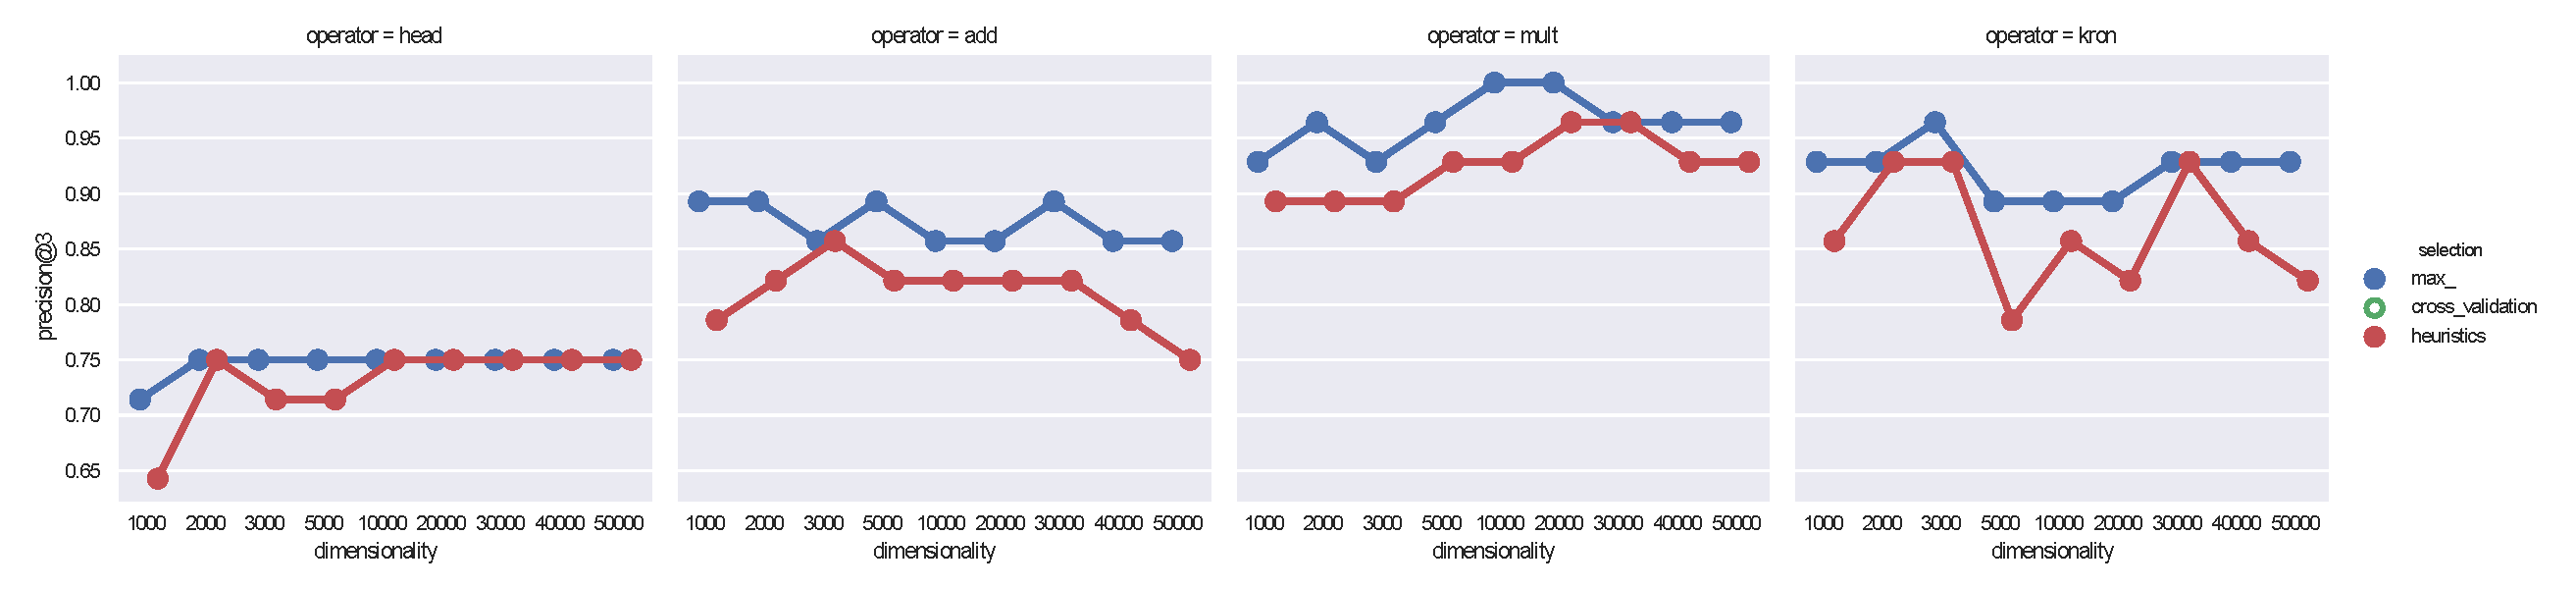
\includegraphics[width=\textwidth]{supplement/figures/phraserel-results}
  \caption{PhraseRel results.}
  \label{fig:phraserel-results}
\end{figure}

%%% Local Variables:
%%% mode: latex
%%% TeX-master: "../thesis"
%%% End:


Figure~\ref{fig:phraserel-results} shows the performance of the models on the PhraseRel dataset. All operators outperform the non-compositional \texttt{head} baseline. Table~\ref{tab:phraserel-max-selection} shows the models that yield the best result together with model parameters.

Multiplication, in general, outperforms all other operators, and with the dimensions of 10000 and 20000 gets the perfect score, giving no support of H\ref{hyp:order}. Model performance weakly depends on the dimensionality for all operators.

Addition and Kronecker achieve the best score with constant frequency, \texttt{head} works best with linear and multiplication with sublinear ($\log n$) frequency.

SPMI is the preferred discriminativeness component for the low-dimensional spaces ($D < 10000$) for \texttt{head}, otherwise, SCPMI is the best behaving \texttt{discr}. For addition and the spaces with $D > 1000$, SPMI is the best, while for the spaces with the same dimensionality multiplication prefers CPMI, which is inline with H\ref{hyp:comp-pmi-cpmi}. Kronecker, most of the times, prefers SCPMI.

\texttt{Head} with dimensions less than 20000 works best with local smoothed context probabilities, however for more dimensional spaces global context probabilities are more competitive. Addition, contrary, prefers smoothed local context probabilities for spaces with dimensions more than 5000. Multiplication exhibits different pattern: when a model contains few dimensions, it prefers local smoothed context probabilities, and for highly-dimensional spaces it prefers local, but unsmoothed context probabilities, contrary H\ref{hyp:cds}. Kronecker is inconsistent with regards to the choice of \texttt{cds}, but models with $D \geq 30000$ global context probabilities perform the best.

Regarding shifting, \texttt{head} prefers sparse spaces $k > 1$, but as dimensionality increases the optimal $k$ values decreases. Addition does not show a consistent behaviour with regard to this parameter. Multiplication, in general, benefits from dense unshifted spaces. Kronecker works best with sparse spaces with increasing sparsity as the dimensionality increases, supporting H\ref{hyp:neg}.

\texttt{Head} benefits from the correlation as the similarity measure, as does multiplication. Addition works best with correlation with spaces $D < 10000$, and with the inner product for more dimensional spaces. Multiplication works best with correlation. Kronecker, for spaces with less than 5000 dimensions, works best with correlation and with the inner product otherwise.

\subsection{Heuristics}
\label{sec:heuristics-phraserel}

\begin{wraptable}[10]{O}{0.5\textwidth}
% \begin{table}[b]
  \vspace{-1em}
  \centering

  \begin{tabular}{lr}
\toprule
      parameter &  partial $R^2$ \\
\midrule
            neg &       0.58 \\
       operator &       0.35 \\
            cds &       0.08 \\
           freq &       0.04 \\
     similarity &       0.03 \\
 dimensionality &       0.03 \\
          discr &       0.02 \\
\bottomrule
\end{tabular}


  \caption{PhraseRel feature ablation}
  \label{tab:phraserel-ablation}
\end{wraptable}


\begin{figure}
% \begin{wrapfigure}{O}{0.5\textwidth}
  % \vspace{-30pt}
  \centering

  \begin{subfigure}[t]{\textwidth}
    \includegraphics[width=1.1\textwidth]{supplement/figures/phraserel-interaction-neg}

  \caption{\texttt{neg}}
  \label{fig:phraserel-neg}
  \end{subfigure}

  \begin{subfigure}[t]{\textwidth}
    \includegraphics[width=1.1\textwidth]{supplement/figures/phraserel-interaction-cds}

  \caption{\texttt{cds}}
  \label{fig:phraserel-cds}
  \end{subfigure}

  \caption{PhraseRel.}
\end{figure}

The linear model achieves an $R^2 = 0.822$. The partial $R^2$ scores are shown on Table~\ref{tab:phraserel-ablation}. The most influential parameters are \texttt{neg}, operator and \texttt{cds}, but the first two have the partial $R^2$ scores much higher then the other parameters. Table~\ref{tab:phraserel-heuristics-selection} shows the performance of the picked models.

\subsubsection{Shifting}
\label{sec:shifting-phraserel}

\texttt{Head} should be used with $k = 1.4$, addition should be used with $k = 2$ and multiplication should be used with $k = 0.5$ (Figure~\ref{fig:phraserel-neg}).

Kronecker has three optimal values of $k$ that is proportional to dimensionality. For models with dimensionality less than 5000, $k = 0.5$ is preferred; for $5000 \geq D < 20000$, the most beneficial choice of \texttt{neg} is $k = 1$; finally, for spaces with more than 20000 dimensions, $k$ should be set to 1.4, which supports H\ref{hyp:neg}.

\subsubsection{Context distribution smoothing}
\label{sec:cont-distr-smooth-phraserel}

The best choice of \texttt{head} is dependant on dimensionality: spaces with less than 10000 dimensions benefit from smoothed local context probabilities ($\alpha = 0.75$) (Figure~\ref{fig:phraserel-cds}). Addition and multiplication work best with global context probabilities, while Kronecker prefers unsmoothed local probabilities ($\alpha = 1$).

\subsubsection{Frequency}
\label{sec:frequency-phraserel}

\begin{figure}[b]
% \begin{wrapfigure}{O}{0.5\textwidth}
  % \vspace{-30pt}
  \centering

  \begin{subfigure}[t]{\textwidth}
    \includegraphics[width=1.1\textwidth]{supplement/figures/phraserel-interaction-freq}

  \caption{\texttt{freq}}
  \label{fig:phraserel-freq}
  \end{subfigure}

  \begin{subfigure}[t]{\textwidth}
    \includegraphics[width=1.1\textwidth]{supplement/figures/phraserel-interaction-similarity}

  \caption{similarity}
  \label{fig:phraserel-similarity}
  \end{subfigure}

  \caption{PhraseRel.}
\end{figure}


\texttt{Head} works best with linear frequency, but the difference with other options is small (Figure~\ref{fig:phraserel-freq}).

Addition benefits from linear frequency, sublinear frequency is very close.

Multiplication works best with sublinear frequency, but linear is very close to it.

Finally, Kronecker works best with $\log n$ with spaces with dimensionality less than 5000, and with linear frequency with more dimensional spaces.

In general, H\ref{hyp:freq} holds, because there is no difference between 1 and $\log n$ choices in model performance.

\subsubsection{Similarity}
\label{sec:similarity-phraserel}

For all operators there is little difference between cosine and correlation, weakly supporting H\ref{hyp:similarity}.

\texttt{Head} works best with correlation as the similarity measure with models with $D < 5000$, and with cosine for more dimensional ones (Figure~\ref{fig:phraserel-similarity}). Note, however, that the difference between the two is very small.

Addition benefits from cosine when $D < 20000$ and from inner product otherwise. But in case of addition, all three similarity measures are close to each others.

Multiplication works best with correlation. Where tested, correlation behaves best with Kronecker.

\subsubsection{Discriminativeness}
\label{sec:discriminativeness-phraserel}

\begin{figure}[b]
% \begin{wrapfigure}{O}{0.5\textwidth}
  % \vspace{-30pt}
  \centering

  \includegraphics[width=1.1\textwidth]{supplement/figures/phraserel-interaction-discr}

  \caption{PhraseRel \texttt{discr}}
  \label{fig:phraserel-discr}
\end{figure}


\texttt{Head} is the only ``operator'' that prefers from different discriminativeness components depending on dimensionality. For models with $D < 5000$, SPMI is the best, while for other dimensions SCPMI is more competitive.

Addition and Kronecker benefit from SPMI, while multiplication from SCPMI, which supports H\ref{hyp:comp-pmi-cpmi}.

\subsection{Difference between Max selection and heuristics on PhraseRel}
\label{sec:diff-phraserel}

Manual parameter selection is more stable than the one based on the maximum values. However in cases where different parameters are picked, there is little or no difference between these parameter choices. For example studied similarity measures yield similar average performance for addition, see Figure~\ref{fig:phraserel-freq}.

Manual heuristics do not pick the best result of 1 (Table~\ref{tab:phraserel-max-selection}), but are close with a multiplicative model with 20000 and 30000 dimensions yielding the score of 0.964 (Table~\ref{tab:phraserel-heuristics-selection}).

The average relative difference between the max selection and the selection based on heuristics is 0.022 for \texttt{head}, 0.072 for addition, 0.041 for multiplication and 0.061 for Kronecker.

Overall, the difference is 0.049, which is within H\ref{hyp:10percent}.

\section{Selected model transfer across the datasets}
\label{sec:select-model-transf-comp}

\subsection{Difference between heuristics}
\label{sec:diff-betw-heur-comp}

There is little agreement on parameter selection based on heuristics among the 3 compositional datasets. The only consistent choice is global context probability (\texttt{cds}) and SCPMI discriminativeness for multiplicative models.

There is more pairwise agreement, for example similarity based on correlation for additive models on KS14 and GS11 and $\log n$ frequency for multiplicative models between GS11 and PhraseRel. The pairwise agreement might be a sign of overfitting, because there is no clear pattern. On the other side, the difference in performance between parameter choices might be neglectable as some parameters consistently show low $R^2$ scores, for example \texttt{discr}. Consequently, there is inconsistency in the hypotheses support.

\subsection{From KS14}
\label{sec:from-ks14}

\begin{figure}[t]
  \centering
    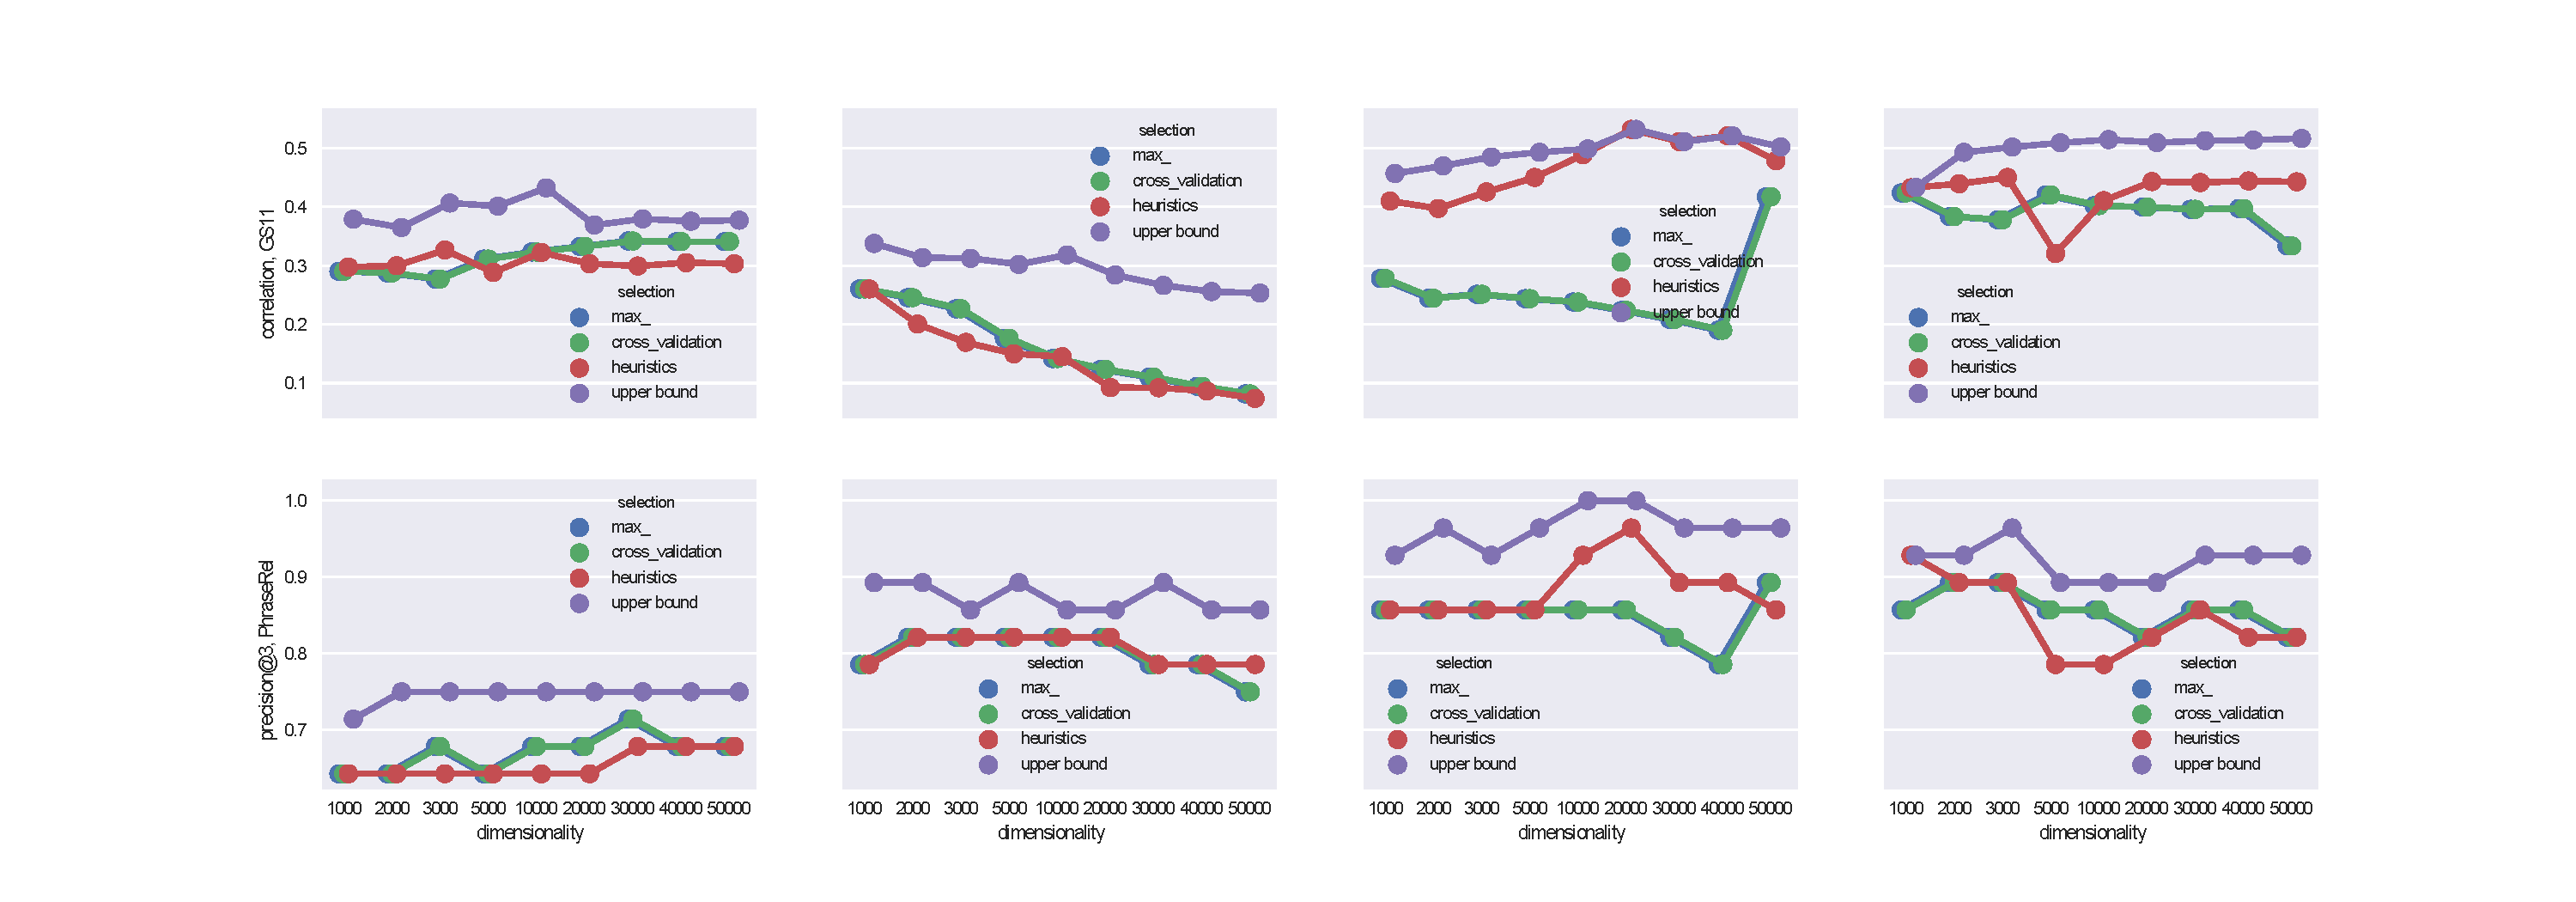
\includegraphics[width=\textwidth]{supplement/figures/KS14-transfer}
    \caption{Transfer from KS14.}
    \label{fig:ks14-transfer}
\end{figure}

%%% Local Variables:
%%% mode: latex
%%% TeX-master: "../thesis"
%%% End:


Figure~\ref{fig:ks14-transfer} show the behaviour of models selected on the KS14 when they are transferred to GS11 and PhraseRel. During the transfer there is little difference in performance between the selection methods, except of multiplicative models where heuristics show better performance and 5000 dimensional Kronecker where heuristics give lower results than the max-based selection.

\todo[noline]{Significance tests}
Heuristic-based selection on average is closer to the upper bound than max based selection, supporting H\ref{hyp:overfitting}. However, both of them are beyond the 10\% boundary set by H\ref{hyp:10percent}. When transferred to GS11 the average difference with the upper bound is 0.335 for max and 0.238 for heuristics. When transferred to PhraseRel the average difference is 0.093 for max and 0.091 for heuristics.

\subsection{From GS11}
\label{sec:from-gs11}

\begin{figure}
  \centering
    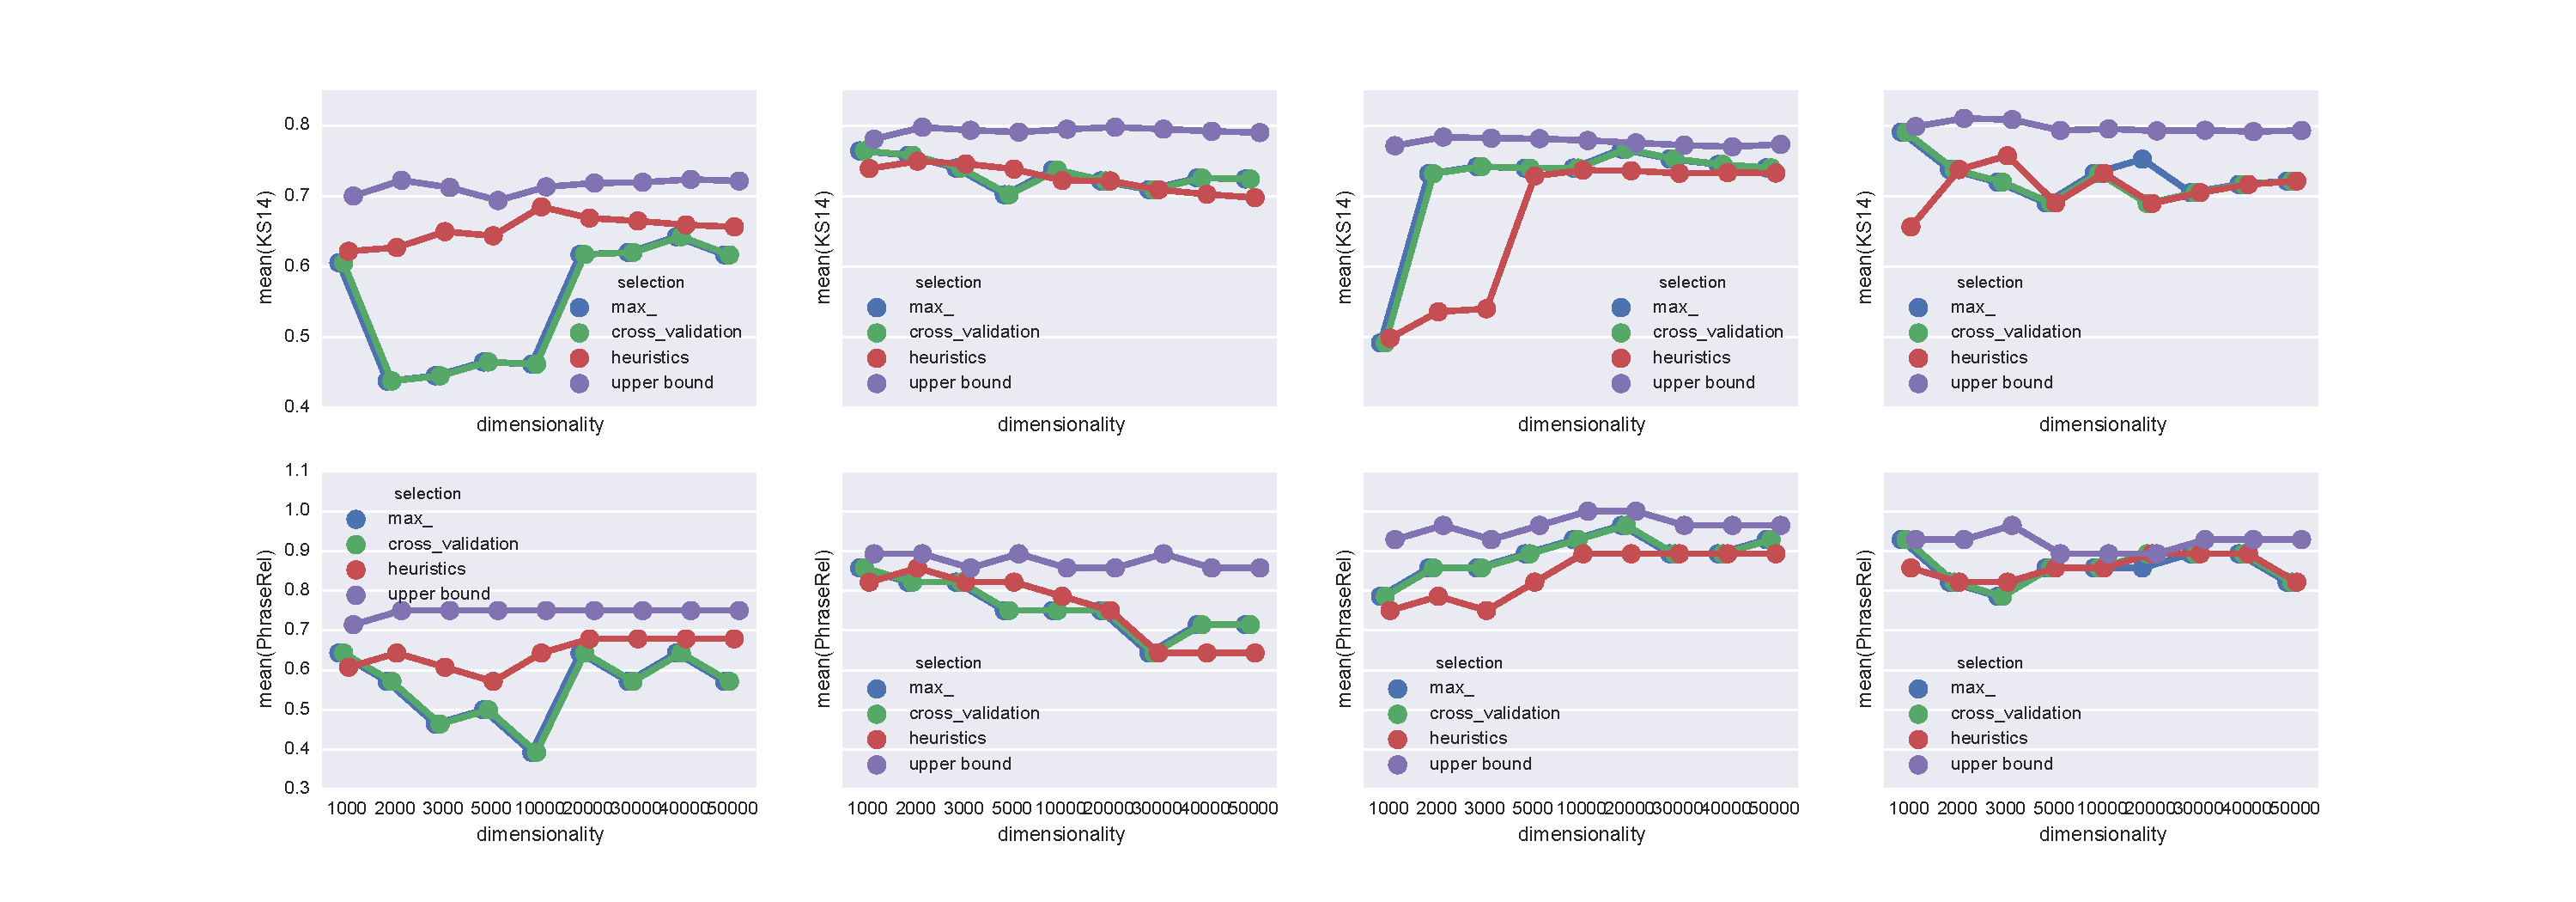
\includegraphics[width=\textwidth]{supplement/figures/GS11-transfer}
    \caption{Transfer from GS11}
    \label{fig:gs11-transfer}
\end{figure}

%%% Local Variables:
%%% mode: latex
%%% TeX-master: "../thesis"
%%% End:


Figure~\ref{fig:gs11-transfer} shows that there is little difference between max and heuristic-based selections. In case of \texttt{head} composition, heuristics lead to higher performance, while for low-dimensional multiplicative models heuristics fall behind the max selection on the KS14 dataset.

\todo[noline]{Significance tests}
When GS11 models are transferred to KS14, the average difference with the upper bound is 0.119 and 0.106 for max and heuristics respectively. For the transfer to PhraseRel, the differences are 0.133 for max and 0.188 for heuristics. Again, the heuristic-based selection outperforms the max based. This supports H\ref{overfitting}, but the results are beyond the limit of H\ref{hyp:10percent}.

\subsection{From PhraseRel}
\label{sec:from-phraserel}

\begin{figure}
  \centering
    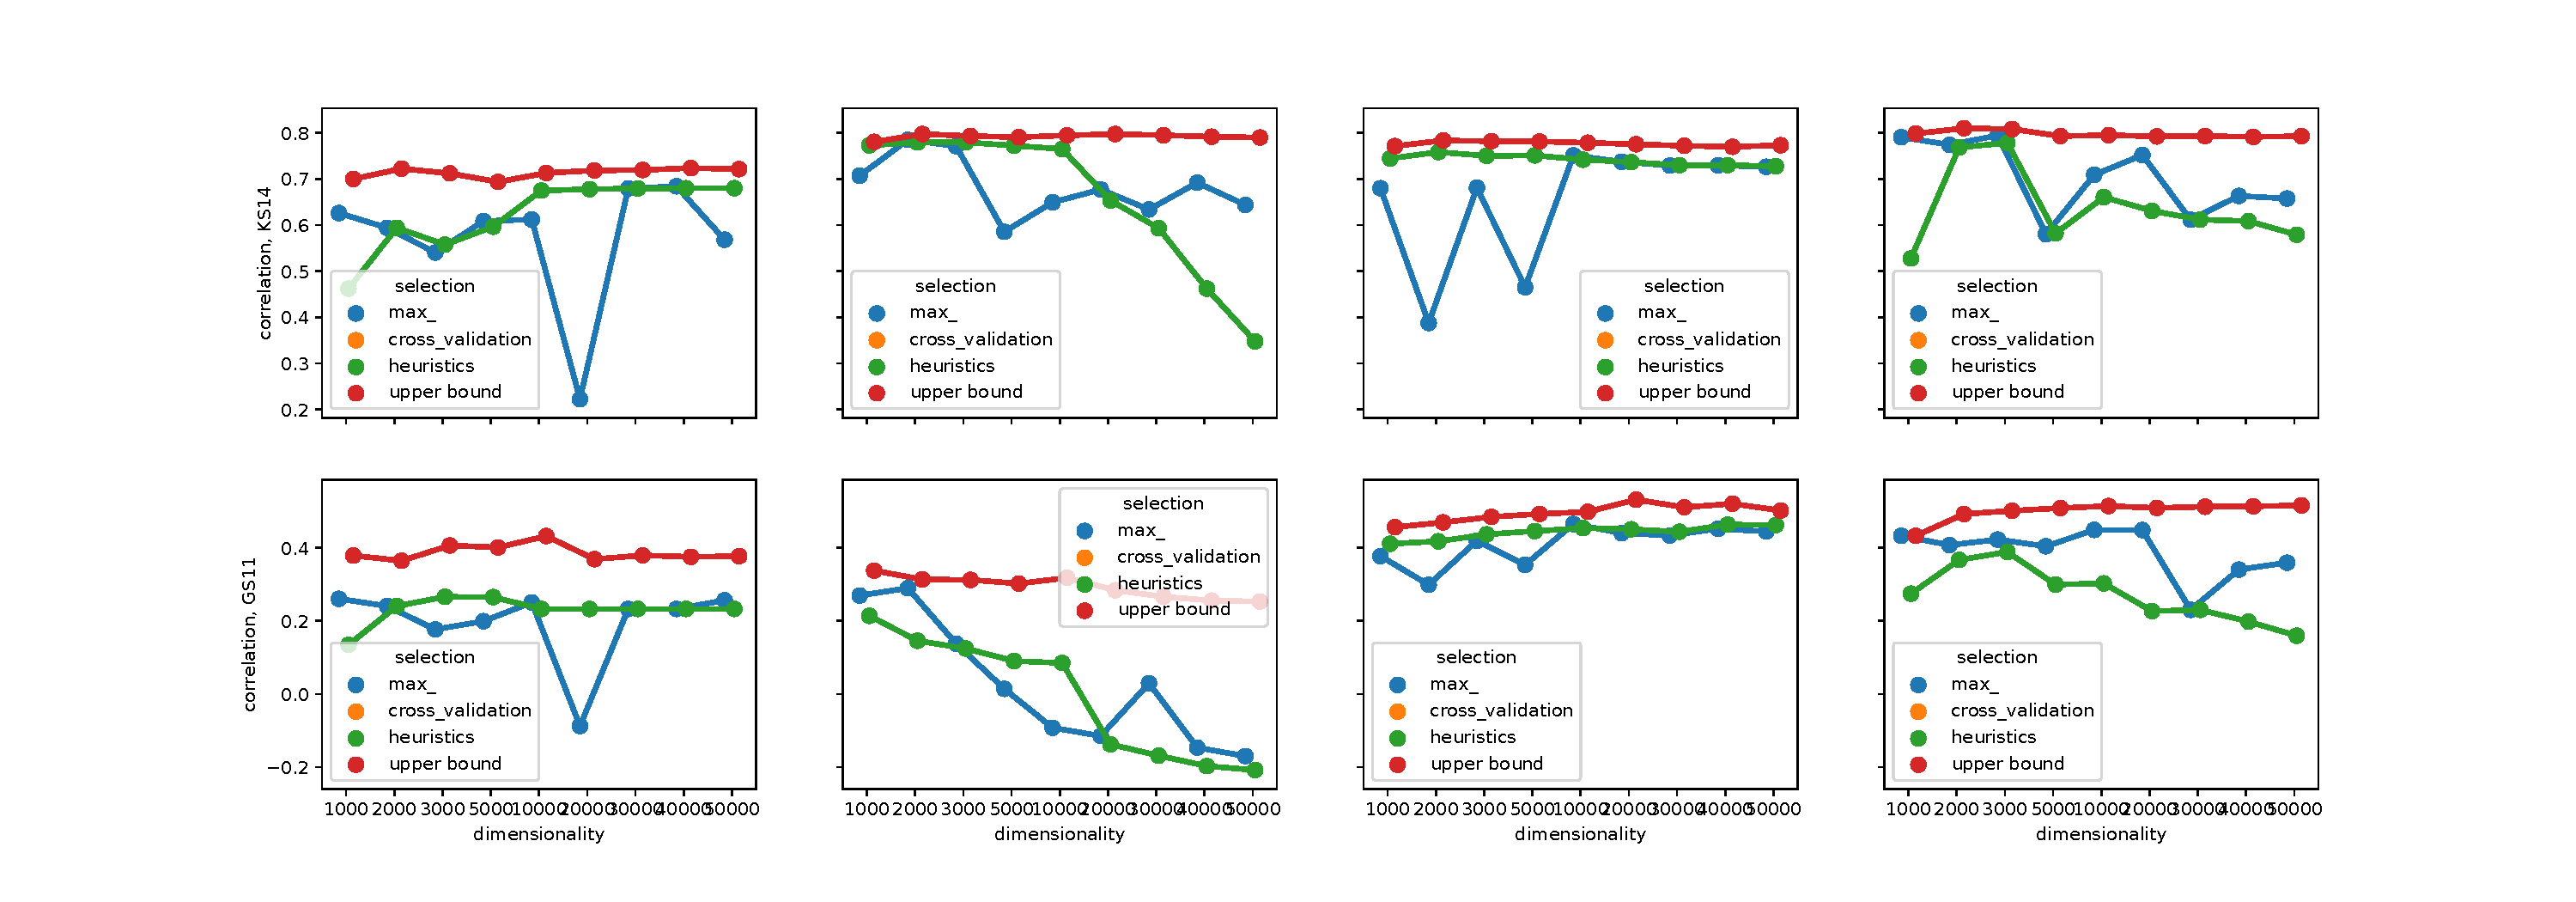
\includegraphics[width=\textwidth]{supplement/figures/PhraseRel-transfer}
    \caption{Transfer from Phraserel.}
    \label{fig:phraserel-transfer}
\end{figure}

%%% Local Variables:
%%% mode: latex
%%% TeX-master: "../thesis"
%%% End:


Figure~\ref{fig:phraserel-transfer} shows that the performance of models based on PhraseRel is less stable, especially for selection by maximum performance.

\todo[noline]{Significance tests}
Transfer to KS14 yields the average differences of 0.152 for max and 0.136 for heuristics. Transfer to GS11 yields the average differences of 0.454 for max and 0.509 for heuristics. Note that the PhraseRel to GS11 transfer is the only case where max selection on average is better than heuristics.

In general, over all compositional datasets, we see---in contrast to the lexical evaluation---that the Max-based selection might be prone to overfitting (H\ref{hyp:overfitting}). However, the result difference is far beyond H\ref{hyp:10percent}, which might be due to the different nature of the tasks: similarity, disambiguation and relevance.

\section{Universal parameter selection for compositional datasets}
\label{sec:robust-param-comp-selecion}

\begin{figure}
  \centering

  \begin{subfigure}[t]{\textwidth}
    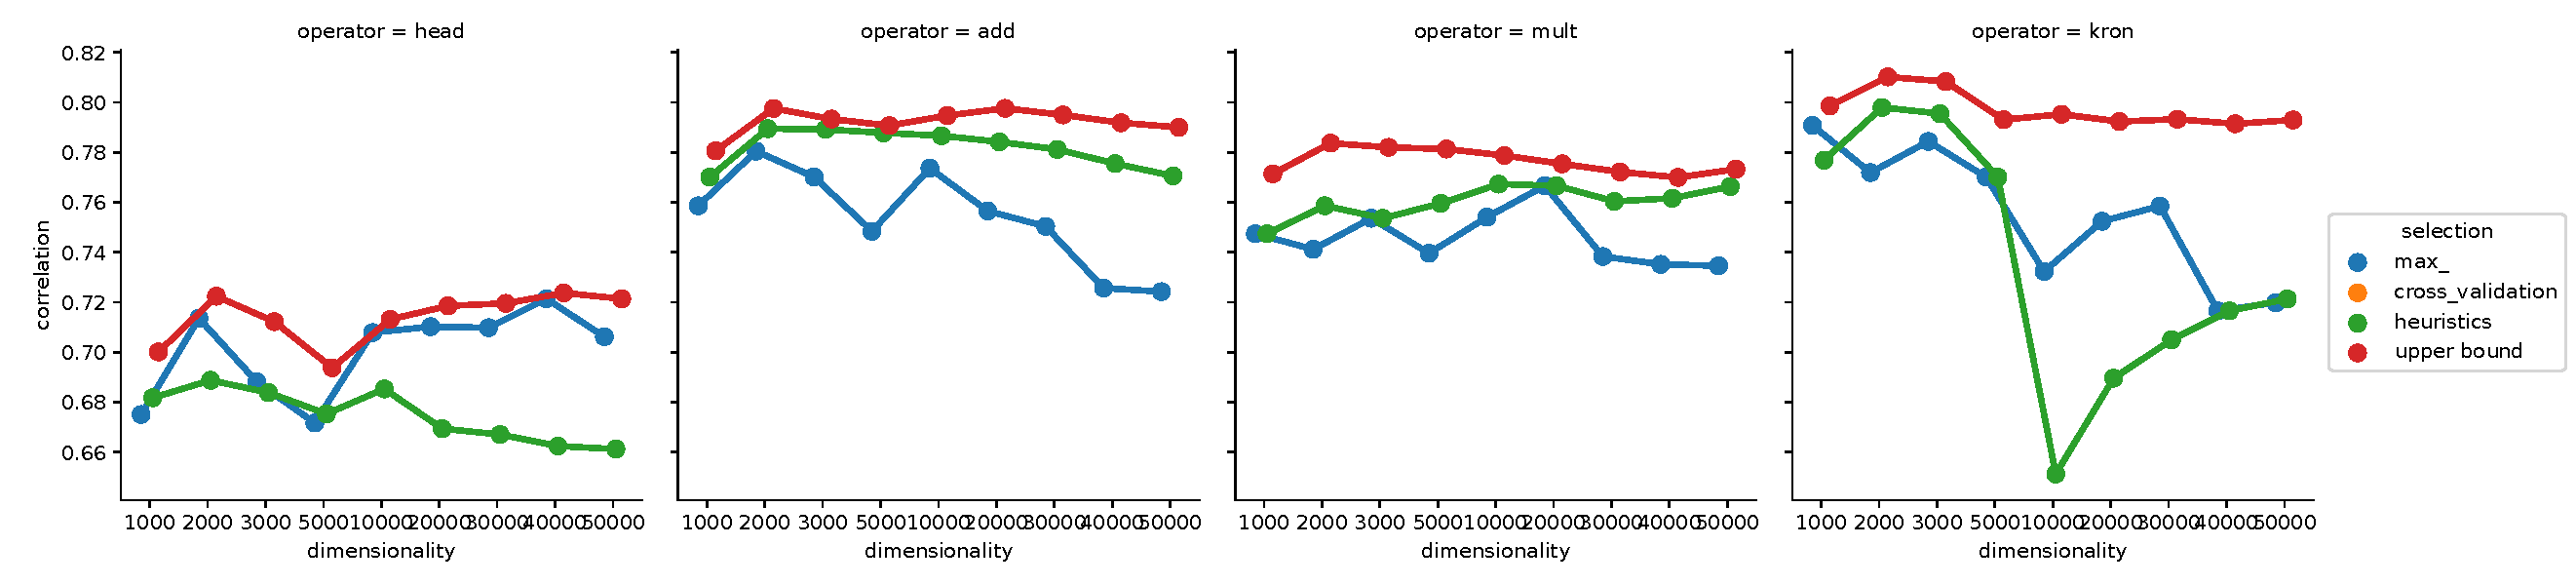
\includegraphics[width=\textwidth]{supplement/figures/compositional-results-ks14}
    \caption{KS14.}
    \label{fig:compositional-results-ks14}
  \end{subfigure}

  \begin{subfigure}[t]{\textwidth}
    \includegraphics[width=\textwidth]{supplement/figures/compositional-results-gs11}
    \caption{GS11.}
    \label{fig:compositional-results-gs11}
  \end{subfigure}

  \begin{subfigure}[t]{\textwidth}
    \includegraphics[width=\textwidth]{supplement/figures/compositional-results-phraserel}
    \caption{PhraseRel.}
    \label{fig:compositional-results-phraserel}
  \end{subfigure}


  \caption{Performance of models based on the selection over the average compositional performance.}
  \label{fig:compositional-results}
\end{figure}

%%% Local Variables:
%%% mode: latex
%%% TeX-master: "../thesis"
%%% End:


Figure~\ref{fig:compositional-results} shows the performance of the models based on the combined selection over the KS14, GS11 and PhraseRel datasets. The combined score is calculated the following way:
$$
\operatorname{score}_\mathit{compositional}(\mathit{model}) =%
\frac{1}{3}%
\frac{\operatorname{score}_\mathit{KS14}(model)}%
{\max_m\operatorname{score}_\mathit{KS14}(m)}%
+%
\frac{1}{3}%
\frac{\operatorname{score}_\mathit{GS11}(model)}%
{\max_m\operatorname{score}_\mathit{GS11}(m)}%
+%
\frac{1}{3}%
\frac{\operatorname{score}_\mathit{PhraseRel}(model)}%
{\max_m\operatorname{score}_\mathit{PhraseRel}(m)}%
$$

The performance of selected models together with the selected parameters is shown on the Table~\ref{tab:compositional-max-selection} (Max selection) and Table~\ref{tab:compositional-heuristics-selection} (selection based on heuristics).

\subsection{Max selection}
\label{sec:max-selection-compositional}

Models with many dimensions not always perform better than their low-dimensional counterparts. Particularly, only \texttt{head} and multiplication benefit from the high number of dimensions. Addition and Kronecker are closer to the upper bound with the dimensionality of few thousands.

\begin{wraptable}[6]{O}{0.5\textwidth}
% \begin{table}
  \vspace{-5em}
  \centering

  \begin{tabular}{lr}
\toprule
      parameter &  partial $R^2$ \\
\midrule
            neg &           0.40 \\
           freq &           0.29 \\
       operator &           0.21 \\
            cds &           0.15 \\
     similarity &           0.08 \\
          discr &           0.06 \\
 dimensionality &           0.05 \\
\bottomrule
\end{tabular}


  \caption{Compositional feature ablation}
  \label{tab:compositional-ablation}
\end{wraptable}


Regarding the hypotheses, there is support of H\ref{hyp:freq} for addition, multiplication and Kronecker, H\ref{hyp:cds} for multiplication and H\ref{hyp:neg} for Kronecker.

\subsection{Heuristics}
\label{sec:heuristics-compositional}

The linear model achieves the $R^2 = 0.769$. Table~\ref{tab:compositional-ablation} shows the partial $R^2$ values for the parameters. The most influential parameters are \texttt{neg}, \texttt{freq} and compositional operator.

\subsubsection{Neg}
\label{sec:neg-compositional}

\begin{figure}
% \begin{wrapfigure}{O}{0.5\textwidth}
  % \vspace{-30pt}
  \centering

  \begin{subfigure}[t]{\textwidth}
    \includegraphics[width=1.1\textwidth]{supplement/figures/compositional-interaction-neg}

  \caption{\texttt{neg}}
  \label{fig:compositional-neg}
  \end{subfigure}

  \begin{subfigure}[t]{\textwidth}
    \includegraphics[width=1.1\textwidth]{supplement/figures/compositional-interaction-freq}

  \caption{\texttt{freq}}
  \label{fig:compositional-freq}
  \end{subfigure}

  \caption{Compositional.}
\end{figure}


For \texttt{head} and models with $D < 10000$ the \texttt{neg} should be set to 1, otherwise it should be 1.4 (Figure~\ref{fig:compositional-neg}).

For addition, 1 is the best choice of \texttt{neg}, but the performance of $k$ values follows H\ref{hyp:neg}.

Multiplication benefits from denser spaces. If the dimensionality is less than 10000, then \texttt{neg} should be set to 0.5, otherwise 0.7 is a good choice, confirming H\ref{hyp:neg}.

Kronecker benefits from the \texttt{neg} of 0.7 if $D < 10000$ and from 1 for the more dimensional cases, supporting H\ref{hyp:neg}. This is similar to multiplication, but Kronecker prefers less dense vectors.

\subsubsection{Freq}
\label{sec:freq-compositional}

$\log n$ is the frequency value of choice of all operators with an exception of multiplication, where the constant frequency is preferred (Figure~\ref{fig:compositional-freq}).

1 behaves good for low-dimensional vector spaces ($D \leq 5000$), giving support of H\ref{hyp:freq}.

\subsubsection{Context distribution smoothing}
\label{sec:cont-distr-smooth-compositional}

\begin{figure}[b]
% \begin{wrapfigure}{O}{0.5\textwidth}
  % \vspace{-30pt}
  \centering

  \begin{subfigure}[t]{\textwidth}
    \includegraphics[width=1.1\textwidth]{supplement/figures/compositional-interaction-cds}

  \caption{\texttt{cds}}
  \label{fig:compositional-cds}
  \end{subfigure}

  \begin{subfigure}[t]{\textwidth}
    \includegraphics[width=1.1\textwidth]{supplement/figures/compositional-interaction-similarity}

  \caption{Similarity}
  \label{fig:compositional-similarity}
  \end{subfigure}

  \caption{Compositional influence of \texttt{cds} and similarity}
\end{figure}


As Figure~\ref{fig:compositional-cds} shows, global context probability is the preferred choice of context probability in all cases, with an exception of Kronecker with $D > 3000$, where smoothed local probabilities are better ($\alpha = 0.75$), supporting H\ref{hyp:cds}.

\subsubsection{Similarity}
\label{sec:similarity-compositional}

Correlation is the dominant choice of the similarity measure (Figure~\ref{fig:compositional-similarity}). However, cosine is preferred in the case of \texttt{head}, with $D > 5000$, and inner product is the only choice for the composition with Kronecker with $D > 3000$.

There is no distinction between cosine and correlation for all compositional operators, which does not contradict H\ref{hyp:similarity}.

\subsubsection{Discr}
\label{sec:discr-compositional}

\begin{figure}
% \begin{wrapfigure}{O}{0.5\textwidth}
  % \vspace{-30pt}
  \centering

  \includegraphics[width=1.1\textwidth]{supplement/figures/compositional-interaction-discr}

  \caption{Compositional influence of \texttt{discr}}
  \label{fig:compositional-discr}
\end{figure}


SPMI is the choice of \texttt{discr} that leads to the best average performance in most cases (Figure~\ref{fig:compositional-discr}). However the difference between SPMI and SCPMI is very small.

The exceptions are Multiplicative composition with $D \geq 10000$ and Kronecker with $D \leq 5000$ where SCPMI outperforms SPMI, as expected by H\ref{hyp:comp-pmi-cpmi}.

\subsection{Comparison with the single dataset beased selections}
\label{sec:comp-with-single-comp}

Manual selection based on a combination of the compositional datasets is more stable with regards to the chosen parameter values than the selection based on the highest values, even though manual selection does not always achieve the performance of Max selection, see Figure~\ref{fig:compositional-results}.

The average difference with the upper bound is 0.040 and 0.041 for Max and heuristics, respectively, when applied to KS14. For GS11, the difference is 0.045 (Max) and 0.127 (Heuristics). For PhraseRel, the difference is 0.055 (Max) and 0.084 (Heuristics).

The numbers are much lower than the transfer of spaces selected on the basis of one dataset (Section~\ref{sec:select-model-transf-comp}. The average normalised difference is within the 10\% limit (H\ref{hyp:10percent}), with an exception of heuristics on GS11. This is an evidence, that there might be one universal model that fits various tasks H\ref{hyp:universal}.

The model selection procedures improve from combination of datasets. One needs to keep in mind that in this case we test model performance on the same dataset as we do parameter selection.

\chapter[Universal model]{Universal model for both lexical and compositional tasks}
\label{sec:universal-param-selection}

\section{Operator dependant (universal) models}
\label{sec:model-selection}

\subsection{Max selection}
\label{sec:max-selection-universal}

Table~\ref{tab:universal-max-selection} shows the performance of the models selected by a combined score of the lexical and compositional datasets. Parameter selection is much more stable than on all previous max-based selections. $\log n$ is a dominant \texttt{freq} choice, cosine is the measure of choice for multiplication and Kronecker, if available. Correlation is the similarity measure for additive composition. Interestingly, if shifting applied, then 1 or 0.7 are chosen as \texttt{neg} values.

\todo[noline]{This is one of the major findings.}
Compositional operator preference depends on the focus of a model.
Addition with many dimensions gives the best results on lexical tasks: 0.384 on SimLex-999 and 0.761 on MEN. Kronecker, on the other side, gives the highest values for compositional datasets: 0.798 on KS14, 0.514 on GS11 and 0.964 on PhraseRel. Multiplication, however, gives the highest ``combined'' score of 0.945, showing that the selection is the closest to the upper bound.

\subsection{Heuristics}
\label{sec:heuristics-universal}

\begin{wraptable}[6]{O}{0.5\textwidth}
  \vspace{-7em}
  \centering

  \begin{tabular}{lr}
\toprule
      parameter &  partial $R^2$ \\
\midrule
           freq &       0.32 \\
            neg &       0.29 \\
     similarity &       0.22 \\
            cds &       0.10 \\
          discr &       0.09 \\
 dimensionality &       0.07 \\
       operator &       0.05 \\
\bottomrule
\end{tabular}


  \caption{Universal (operator dependent) feature ablation}
  \label{tab:universal-ablation}
\end{wraptable}


Performance of the models selected manually shown on Table~\ref{tab:universal-heuristics-selection}. Again, there is a lot consistency between parameters. The linear model achieves $R^2 = 0.828$. The most influencing parameters are \texttt{freq}, \texttt{neg} and a similarity measure, refer to Table~\ref{tab:universal-ablation}.

Heuristics for addition choose models that score the highest on lexical tasks: 0.384 on SimLex-999 and 0.764 on MEN (Table~\ref{tab:universal-heuristics-selection}). Moreover, with more than 20000 dimensions there is no difference between the selection procedures (Max or heuristics) of the additive and Kronecker-based models.

Kronecker is strong in compositional tasks scoring 0.795 on KS14, 0.516 on GS11 and 0.929 on PhraseRel (Table~\ref{tab:universal-heuristics-selection}).

Multiplication, again, is a compromise between the two: it gives the highest combined score of 0.941. The highest Kronecker's combined is 0.913, while addition's highest score is only 0.843.

\subsection{Comparison}
\label{sec:comparison-universal}

\begin{figure}
  \centering
  \begin{subfigure}[t]{\textwidth}

    \includegraphics[width=\textwidth]{supplement/figures/universal-results-simlex999}
    \caption{SimLex999.}
    \label{fig:universal-results-simlex}
  \end{subfigure}

  \begin{subfigure}[t]{\textwidth}
    \includegraphics[width=\textwidth]{supplement/figures/universal-results-men}
    \caption{MEN.}
    \label{fig:universal-results-men}
  \end{subfigure}


  \begin{subfigure}[t]{\textwidth}
    \includegraphics[width=\textwidth]{supplement/figures/universal-results-ks14}
    \caption{KS14.}
    \label{fig:universal-results-ks14}
  \end{subfigure}

  \begin{subfigure}[t]{\textwidth}
    \includegraphics[width=\textwidth]{supplement/figures/universal-results-gs11}
    \caption{GS11.}
    \label{fig:universal-results-gs11}
  \end{subfigure}

  \begin{subfigure}[t]{\textwidth}
    \includegraphics[width=\textwidth]{supplement/figures/universal-results-phraserel}
    \caption{PhraseRel.}
    \label{fig:universal-results-phraserel}
  \end{subfigure}


  \caption{Performance of models based on the selection over the average universal performance.}
  \label{fig:universal-results}
\end{figure}

%%% Local Variables:
%%% mode: latex
%%% TeX-master: "../thesis"
%%% End:


On lexical tasks, there is little difference between the model selection methods especially for spaces with more than 30000 dimensions, as Figures~\ref{fig:universal-results-simlex} and \ref{fig:universal-results-men} show.

On compositional tasks, dimensionality does not contribute as much as in case of lexical tasks, with an exception of addition on the GS11 dataset, where performance decreases as dimensionality increases.

\todo[noline]{One of the major findings.}
When the models that are selected on lexical tasks are applied in a compositional setting, they perform worse than the models selected based on the universal score. This suggests that a model that is good on lexical tasks will not necessarily perform well on a compositional task. In addition, sometimes this difference increases as dimensionality increases, for example this is the case for multiplication, the most notable difference is observed on KS14 (Figure~\ref{fig:universal-results-ks14}).

\todo[inline]{Compare the average differences of every dataset.}

\section{Operator independant universal models}

\todo[inline]{We have seen in the previous section that even though parameter selection is different between operators, there are choices that are shared. Given this and the fact that the difference between some of the choices is marginal, we try to look for truly universal parameters.}

\subsection{Max selection}
\label{sec:max-selection-single}

Table~\ref{tab:single-max-selection} shows \todo{describe how it was combined} the combined score for all datasets abstracting over a compositional operator.

The parameter selection shows a clear pattern. \texttt{freq} shows a clear pattern: low-dimensional spaces perform best with 1 as the frequency choice, while high dimensional models perform better with $\log n$. Cosine is a better suited similarity measure for models with few dimensions, correlation with many. Finally, global context probabilities are the best in a low-dimensional case, while local context probabilities perform best with many dimensions.

\todo[inline]{Average difference with the upper bound.}

\subsection{Heuristics}
\label{sec:heuristics-single}

Heuristics in general repeat the parameter selection choice, but the switch happens with more dimensions (at 20000, not at 5000) refer to Table~\ref{tab:single-heuristics-selection} for the results and Figure~\ref{fig:single-params} for the parameter behavior.

\begin{wraptable}[10]{O}{0.5\textwidth}
%\begin{table}[b]
  % \vspace{-2em}
  \centering

  \begin{tabular}{lr}
\toprule
      parameter &  partial $R^2$ \\
\midrule
           freq &   0.434 \\
     similarity &   0.269 \\
            neg &   0.196 \\
          discr &   0.092 \\
            cds &   0.090 \\
 dimensionality &   0.034 \\
\bottomrule
\end{tabular}


  \caption{Universal (operator-independent) feature ablation}
  \label{tab:single-ablation}
  % \end{wraptable}
\end{wraptable}

The linear model gives $R^2 = 898$. The most influential parameters are \texttt{freq}, similarity measure and \texttt{neg}, refer to Table~\ref{tab:single-ablation}.

% \begin{wrapfigure}{O}{0.5\textwidth}
\begin{figure}[b]
  % \vspace{-30pt}
  \centering

  \begin{subfigure}[t]{0.49\textwidth}
  \includegraphics[width=\textwidth]{supplement/figures/single-interaction-freq}

  \caption{\texttt{freq}}
  \label{fig:single-freq}
  \end{subfigure}
  \begin{subfigure}[t]{0.49\textwidth}

  \includegraphics[width=1.1\textwidth]{supplement/figures/single-interaction-similarity}

  \caption{Similarity measure}
  \label{fig:single-similarity}
  \end{subfigure}

  \begin{subfigure}[t]{0.49\textwidth}

  \includegraphics[width=\textwidth]{supplement/figures/single-interaction-neg}

  \caption{\texttt{neg}}
  \label{fig:single-neg}
  \end{subfigure}
  \begin{subfigure}[t]{0.49\textwidth}

  \includegraphics[width=\textwidth]{supplement/figures/single-interaction-discr}

  \caption{\texttt{discr}}
  \label{fig:single-discr}
  \end{subfigure}

  \begin{subfigure}[t]{0.49\textwidth}

  \includegraphics[width=\textwidth]{supplement/figures/single-interaction-cds}

  \caption{\texttt{cds}}
  \label{fig:single-cds}
  \end{subfigure}

  \caption{Universal (parameter independent) parameter influence}
  \label{fig:single-params}
\end{figure}


% \subsubsection{Tweaked IR evaluation}
% \label{sec:tweak-ir-eval}

% \todo[inline]{Discuss \cite{Milajevs:2015:IMN:2808194.2809448} and link to \ref{sec:phraserel}}

% \section{PhraseRel: relevance of sentences}
% \label{sec:sentential-relevance}

%%% Local Variables:
%%% mode: latex
%%% TeX-master: "thesis"
%%% End:
